\partimage[width=0.8\columnwidth]{Figures/PartImages/FigCh3.png}
\part{Le moment angulaire orbital dans la génération d'harmoniques d'ordre élevé}
\label{PA:OAM_HHG}
\chapternonum{Introduction}
La GHOE est un phénomène aujourd'hui bien compris et qui a été longuement étudié en fonction de nombreux paramètres : intensité, pression, longueur d'onde, etc. Toutefois, mis à part quelques travaux numériques sur les faisceaux de Bessel \mycite{augustepra2008}, la GHOE à partir de faisceaux portant du MAO n'a été que très peu étudiée. 

Dans ce chapitre nous décrirons en détail le processus de GHOE à partir de faisceaux de Laguerre-Gauss, qui comme on l'a vu dans la partie \ref{sec:oamLG} sont des modes propres du moment angulaire orbital. Nous commencerons par décrire le dispositif expérimental développé à cet effet, avant de présenter les résultats obtenus. Ces résultats seront ensuite interprétés et comparés à des calculs analytiques et numériques, qui montreront que le moment angulaire orbital de la lumière est conservé dans la GHOE.

Une fois le moment angulaire orbital harmonique caractérisé, nous nous intéresserons à la structure spatio-temporelle du rayonnement. Enfin, nous étudierons expérimentalement et théoriquement le rôle des trajectoires quantiques dans la GHOE à partir de faisceaux de Laguerre-Gauss. On montrera qu'elles permettent de contrôler le nombre quantique radial des modes émis, en plus du nombre quantique azimutal. 
\newpage

\chapter{Profils spatiaux d'harmoniques d'ordre élevé obtenues à partir d'un faisceau de Laguerre-Gauss}
Dans ce chapitre nous détaillerons d'abord la méthode que nous avons choisie pour générer des modes de LG dans le domaine visible. Nous détaillerons ensuite le dispositif XUV retenu pour imager spatialement les harmoniques produites. Finalement, nous présenterons les spectres obtenus. Leur analyse, qui requiert un appareil théorique, sera exposée au chapitre suivant.

\section{Génération de modes de Laguerre-Gauss dans le visible}
L'expression d'un mode de Laguerre-Gauss a été donnée au chapitre précédent (équation \ref{eq:lgmodes}). Ils sont décrits par deux indices, $\ell$ et $p$. Dans un premier temps, nous nous focalisons sur le premier, qui détermine le moment angulaire orbital porté par le faisceau. Il apparaît effectivement dans le terme de phase hélicoïdale $e^{\rmi\ell\theta}$. Nous ici deux techniques de génération de ces faisceaux dans le domaine visible ou proche infrarouge.

\subsection{Techniques de génération de modes de LG}
\subsubsection{Superposition de modes de Hermite-Gauss}
\label{sec:hg_modes}
Les faisceaux de LG étant des modes du champ électromagnétique, on peut d'abord penser à modifier le laser lui-même pour qu'il lase directement dans le mode désiré. En introduisant des éléments absorbants dans la cavité, il est a priori possible d'interdire la génération d'un mode Gaussien. En pratique, il est assez compliqué de sélectionner un mode de LG. Il est par contre assez simple de sélectionner un des modes de \textit{Hermite-Gauss}, qui sont les solutions de l'équation d'onde en coordonnées cartésiennes, comme on l'a montré à la partie \ref{sec:HGmodes}. Ces modes sont souvent appelés modes $\mbox{TEM}_{nm}$, pour "Transverse Electro-Magnetic", dont le mode Gaussien $\mbox{TEM}_{00}$ n'est simplement que le mode d'index le plus bas. En insérant simplement un fil vertical (resp. horizontal) dans la cavité laser, on bloque la génération du $\mbox{TEM}_{00}$ et on obtient un mode $\mbox{TEM}_{01}$ (resp. $\mbox{TEM}_{10}$).

Les faisceaux de Hermite-Gauss constituent également une base orthonormée des modes du champ, dans laquelle on peut écrire les modes de Laguerre-Gauss. On peut montrer \mycite{BeijersbergenOC1993} que les composantes du mode $\mathcal{LG}_{\ell,p}$ sont égales aux composantes d'un mode $\mbox{TEM}_{nm}$ incliné à 45\degres{} avec $p = \mathrm{min}(m,n)$ et $\ell=m-n$, la seule différence étant l'ajout d'une phase de $\pi/2$ entre les différentes composantes successives. Par exemple pour $\ell = 1$,
\begin{align*}
\mbox{TEM}_{n,m}^{45\mbox{\degres}}&=\frac{1}{\sqrt{2}}\mbox{TEM}_{01}+\frac{1}{\sqrt{2}}\mbox{TEM}_{10} \mbox{ et}\\
\mathcal{LG}_{1,0}&=\frac{1}{\sqrt{2}}\mbox{TEM}_{01}+\frac{\rmi}{\sqrt{2}}\mbox{TEM}_{10}.
\end{align*}
Pour $\ell = 2$, 
\begin{equation*}
\mathcal{LG}_{2,0}=\frac{1}{2}\mbox{TEM}_{02}+\frac{\rmi}{\sqrt{2}}\mbox{TEM}_{11}-\frac{1}{\sqrt{2}}\mbox{TEM}_{20}
\end{equation*}
et ainsi de suite.
Comme dit plus haut, il est possible de générer un mode $\mbox{TEM}_{n,m}$ en cavité, il reste seulement à l'incliner à 45\degres par rapport au repère choisi. Pour contrôler la phase entre les composantes relatives, les auteurs de \mycite{BeijersbergenOC1993} ont montré qu'on pouvait utiliser des lentilles cylindriques. En effet, une lentille cylindrique convergente ne focalise qu'une seule des composantes cartésiennes, qui va subir un déphasage au passage du foyer dû à la phase de Gouy. On recollimate ensuite le faisceau avec une deuxième lentille cylindrique de même focale $f$. La phase ajoutée est ajustée en changeant la distance entre ces deux lentilles; pour obtenir $\pi/2$ il faut choisir $\sqrt{2}f$. La Figure \ref{Fig:Modeconv} illustre le principe de ce dispositif, appelé convertisseur de mode, très utilisé dans la communauté.

\begin{figure}[!ht]
\centering
\def\svgwidth{0.5\columnwidth}
\import{Figures/Mode_Converter/}{mode_converter.pdf_tex}
\caption{Schéma de fonctionnement d'un convertisseur de mode : en partant d'un $\mbox{TEM}_{01}$ incliné à 45\degres, on obtient un mode $\mathcal{LG}_{1,0}$. Tiré de \mycite{PadgettAllen1999}.}
\label{Fig:Modeconv}
\end{figure}

L'intérêt de ce dispositif est de créer des modes purs : on obtient exactement le faisceau de Laguerre-Gauss recherché. Il présente cependant deux inconvénients : (1) il faut disposer d'un mode $\mbox{TEM}_{0\ell}$ au départ, ce qui devient compliqué dès que $\ell$ augmente. De plus, il est peu pratique de devoir modifier la cavité laser, particulièrement dans le cas des lasers de puissances utilisés pour la HHG. (2) Le faisceau est focalisé dans une dimension entre les deux lentilles. La puissance fournie par notre laser imposerait de réaliser la conversion dans une enceinte à vide, sans quoi la focalisation dans l'air détruirait le profil spatial et temporel du faisceau. Pour ces raisons, nous avons choisi une méthode plus flexible et plus adaptée à un laser de puissance.

\subsubsection{Utilisation d'une lame de phase à spirale}
Cette technique est probablement la façon la plus intuitive d'ajouter le terme de phase qui nous intéresse au faisceau. Pour rajouter une phase $e^{\rmi\ell\theta}$, il suffit d'utiliser une lame de verre transparente dont l'épaisseur varie proportionnellement à $\theta$. On forme ainsi une \textit{lame de phase à spirale} (Spiral Phase Plate, SPP), concept proposé dans \mycite{BeijersbergenOC1994} et représenté sur la Figure \ref{Fig:SPP}.\par
\begin{figure}[!ht]
\centering
\def\svgwidth{0.5\columnwidth}
\import{Figures/SPP/}{SPP.pdf_tex}
\caption{Lame de phase à spirale. La flèche rouge représente le trajet d'un rayon optique. Adapté de \mycite{YaoAOP2011}.}
\label{Fig:SPP}
\end{figure}
La lame présente une discontinuité pour $\theta=0$\degres, dont la hauteur h permet de contrôler le moment angulaire orbital transféré au faisceau pour une longueur d'onde donnée. Si cette hauteur est assez faible pour que l'on reste dans le régime paraxial, on peut considérer que la lame agit uniquement sur la phase du faisceau incident. Ainsi si on choisit 
\begin{equation*}
h = \frac{\ell\lambda}{n-1},
\end{equation*}
où $n$ est l'indice de réfraction du milieu, pour un champ d'entrée $u(r,\theta,z)$ on obtient directement après la lame $u' = u\exp{(-\rmi \ell \theta)}$.	Il est donc non seulement possible de passer d'un mode Gaussien à un mode Laguerre-Gaussien, mais encore de changer l'indice d'un mode déjà Laguerre-Gaussien.\par
La lame de phase illustre de façon intuitive la création de MAO : si on considère une onde plane arrivant perpendiculairement à la surface plane de la lame, le rayon qui sort de la lame sera dévié par réfraction à travers la surface hélicoïdale. Cette réfraction se fait dans la direction azimutale, le moment linéaire de la lumière acquière donc une composante azimutale, synonyme de moment angulaire. Plus précisément, pour un rayon $r$ donné, l'angle de la surface	vaut $h/(2\pi r)$. Si on applique la loi de Snell-Descartes on obtient que le rayon est dévié d'un angle $\alpha = (n-1)\ell\lambda/(2\pi r(n-1)) = \ell/(k_0r)$. Le moment linéaire par photon vaut $\hbar k_0$, donc le moment angulaire par photon vaut $r\times\hbar k_0\times\ell/(k_0r) = \ell\hbar$.


Si le principe d'une SPP est simple, sa construction est beaucoup plus compliquée. Les tolérances sur la valeur de h et la régularité de la surface sont très strictes aux longueurs d'ondes optiques, sans quoi la qualité du mode de sortie sera détériorée (si h n'est pas adapté, on peut même créer des modes d'indice non entier, cf. \mycite{LeachNJP2004}). D'ailleurs, lors des premiers travaux sur le sujet (\mycite{BeijersbergenOC1994}), la température de la lame était ajustée pour accorder précisément la hauteur de la lame à la longueur d'onde. La technique a évolué et il est maintenant possible de créer des SPP de très bonne qualité \mycite{OemrawsinghAO2004}.

Enfin, remarquons que même pour une SPP parfaite, la conversion d'un mode à l'autre n'est jamais idéale. La SPP agit sur la phase du faisceau, mais ne modifie pas le profil d'intensité. Ainsi, à sa sortie le champ électrique a la bonne phase mais pas la distribution d'intensité d'un mode de Laguerre-Gauss (termes sur la première ligne de l'équation \ref{eq:lgmodes}). La conséquence est que le champ $u_{exp}$ créé n'est pas un mode pur du champ, mais une superposition de modes de Laguerre-Gauss de différents indices. Ainsi, son intensité sera fortement modulée au cours de la propagation selon la phase entre ces différents modes. Le cas qui nous intéresse principalement est la conversion d'un mode Gaussien vers un mode LG. Dans ce cas, cette superposition s'écrit :
\begin{align}
\begin{split}
u_{exp}(r,\theta,z) &= \sum_{p=0}^\infty\sum_{\ell=-\infty}^\infty{\Braket{u_{exp}(r,\theta,z)|\mathcal{LG}_{\ell,p}(r,\theta,z)} \ket{\mathcal{LG}_{\ell,p}(r,\theta,z)}}\\
&=\sum_{p=0}^\infty\sum_{\ell=-\infty}^\infty{\Braket{TEM_{00}(r,\theta,z)\cdot e^{\rmi\ell'\theta}|\mathcal{LG}_{\ell,p}(r,\theta,z)} \ket{\mathcal{LG}_{\ell,p}(r,\theta,z)}},
\end{split}
\label{Eq:decompLG}
\end{align}
où $\ell'$ est l'indice azimutal correspond à la hauteur de la SPP. Les coefficients sont simplement donnés par le produit scalaire ci-dessus. On remarque qu'il a la forme suivante :
\begin{equation*}
\Braket{TEM_{00}(r,\theta,z)\cdot e^{\rmi\ell'\theta}|\mathcal{LG}_{\ell,p}(r,\theta,z)} = \int_{r=0}^\infty\int_{\theta=0}^{2\pi}{\ldots \; e^{\rmi(\ell'-\ell)\theta}r\rmd r \rmd \theta},
\end{equation*}
l'intégrale selon $\theta$ s'annule donc dès que $\ell\neq\ell'$. Les modes de la superposition ont donc tous le même index azimutal mais des $p$ différents. Ces coefficients peuvent être calculés numériquement, par exemple \mycite{BeijersbergenOC1994} obtiennent pour le cas $\ell' = 1$ les valeurs présentées dans le Tableau \ref{Tab:DecompBei}. On conclut donc que le faisceau est composé majoritairement du mode $\mathcal{LG}_{1,0}$. Les valeurs deviennent moins bonne lorsqu'on augmente $\ell$, par exemple un Gaussien passant à travers une lame dessinée pour ajouter $\Delta\ell =2$ n'est composé qu'à 50\% du mode $\mathcal{LG}_{2,0}$ recherché.
\begin{center}
  \begin{tabular}{| c | c | c | c | c | c | c |}
    \hline
		& $p = 0$ & 1 & 2 & 3 & 4 & 5 \\ \hline
    $\ell=1$ & 78.5 & 9.82 & 3.68 & 1.92 & 1.17 & 0.79 \\ \hline
  \end{tabular}
	\caption{Décomposition du champ obtenu en passant un mode Gaussien pur à travers une lame de phase à spirale. D'après \mycite{BeijersbergenOC1994}.}
	\label{Tab:DecompBei}
\end{center}
Pour finir, mentionnons une technique permettant de relâcher un peu les contraintes de fabrication d'une SPP : il est possible de discrétiser la pente de phase, ce qui rend la lame plus facile à construire et donc plus accessible. Cette technique est détaillée dans \mycite{SuedaOE2004}, où les auteurs calculent l'influence du nombre de points de discrétisation sur la pureté modale obtenue :
\begin{center}
  \begin{tabular}{| c | c | c | c | c | c |}
    \hline
		Nombre de points de discrétisation & $\infty$ & 32 & 16 & 8 & 4 \\ \hline
    Efficacité $\mathcal{LG}_{0,0}\rightarrow\mathcal{LG}_{1,0}$ & 78.5 & 78.3 & 77.5 & 74.6 & 63.7 \\ \hline
  \end{tabular}
	\caption{Efficacité de conversion d'une lame de phase à spirale $\Delta\ell=1$ en fonction du niveau de discrétisation. D'après \mycite{SuedaOE2004}.}
	\label{Tab:DecompSueda}
\end{center}
La qualité du mode obtenue est donc très correcte même jusqu'à 8 niveaux. Les auteurs montrent également que ces lames de phase sont adaptées à des utilisations avec des faisceaux courts et intenses, contrairement à la plupart des autres méthodes. Pour ces raisons, nous avons finalement choisi d'utiliser une lame de phase discrétisée sur 16 niveaux, et disposons de lames $\Delta\ell = 1$ et $\Delta\ell = 2$ à 800 nm, ce qui nous permet d'aller jusqu’à $\ell = 3$ en les mettant l'une après l'autre.

\subsection{Résultats expérimentaux sur la création de modes de Laguerre-Gauss dans l'infrarouge}
\label{sec:spp}
Le système laser a été décrit au chapitre \ref{sec:laser}. Notons encore une fois l'importance du filtrage spatial installé sur notre chaîne : il nous garantit un mode Gaussien très pur, ce qui favorise grandement la création de modes Laguerre-Gaussien de qualité. \par
Les lames de phase utilisées ont été construites par la société Silios Technologies et font 17 mm de diamètre. Elle ou elles sont insérées directement après l'iris et avant la lentille. Le faisceau étant collimaté, nous n'avons pas observé de différence notable selon le placement de la lame. Il est intéressant d'observer l'intensité du faisceau un peu après le passage dans la lame, présentée sur la figure \ref{Fig:BeamAfterSPP}.

\begin{figure}[!ht]
\centering
\def\svgwidth{0.4\columnwidth}
\import{Figures/SPP/}{Beam_1m_After_SPP.pdf_tex}
\caption{Intensité transverse après être passée dans une lame de phase à spirale $\Delta\ell = 1$. Le faisceau est d'abord diaphragmé par un iris de diamètre 10 mm, la distance d'observation après la lame est de 1 m.}
\label{Fig:BeamAfterSPP}
\end{figure}

On observe 16 ``pétales'' sur les bords du faisceau, qui correspondent à la diffraction par les 16 marches de la lame. On voit également la singularité de phase déjà formée, qui donne un zéro d'intensité au centre. Clairement, l'intensité du faisceau est encore très loin de celle d'un mode de Laguerre-Gauss : il n'y a que dans le champ lointain que le faisceau prendra la forme désirée. Dans notre cas, cela se passe au foyer de la lentille de génération. Nous imageons ce foyer à l'aide d'une caméra CCD Imagine Source équippée d'un objectif x5 et d'un tube de 160 mm. La figure \ref{Fig:LGFocus} présente les résultats obtenus.\par
\begin{figure}[!ht]
\centering
\def\svgwidth{0.8\columnwidth}
\import{Figures/IRFocus/}{SPP1focus.pdf_tex}
\caption{Intensité laser au foyer d'une lentille de 1m, après passage à travers (1) une lame de phase $\Delta\ell = 1$, (2) une lame de phase $\Delta\ell = 2$, et (3) les deux lames placées successivement.}
\label{Fig:LGFocus}
\end{figure}
On mesure le diamètre de l'anneau, défini comme la distance entre les deux maxima d'intensité le long d'une ligne radiale, et on obtient 200, 280 et 400 \si{\um} pour $\ell=$1, 2, 3. Ceci est cohérent avec la dépendance en $\sqrt{\ell}$ attendue (voir équation \ref{Eq:rmax_LG}). Pour mesurer le MAO porté par le faisceau, il existe de nombreuses techniques développées dans le domaine visible et infrarouges dont le but est toujours de révéler le terme de phase $\mathrm{e}^{\rmi\ell\theta}$. Pour cela, il est naturel d'essayer d'observer des interférences, soit avec un autre faisceau - l'interférence avec un gaussien donne une ``fourche'' d'ordre $\ell$ \mycite{bazhenov1990} - ou bien du faisceau avec lui même, c'est-à-dire sa diffraction. De nombreux objets diffractifs ont été utilisés, par exemple une fente \mycite{ghai2009} ou des fentes de Young \mycite{sztul2006}, avec lesquelles le signe et la parité de $\ell$ se retrouvent dans le décalage des franges, ou bien des objets plus compliqués tels que des grilles de pupilles \mycite{berkhout2008} qui donnent directement la valeur de $\ell$. On peut également mentionner les ouvertures bloquant une partie angulaire du faisceau, ce qui se répercute sur le contenu modal du faisceau à travers la relation d'incertitude $\Delta\ell\Delta\phi > K$ déjà mentionnée (\textcolor[rgb]{1,0,0}{rajouter au chapitre 2}). Certaines méthodes sont généralisables au cas d'un photon unique et ont permis de mesurer de l'intrication entre différents états de moment orbital angulaire \mycite{MairNature2001} ainsi qu'un équivalent angulaire au paradoxe EPR \mycite{LeachScience2010}. \par 
Nous avons choisi d'utiliser une ouverture en triangle, qui donne une figure de diffraction assez surprenante : on obtient une grille de points diffractés en forme de triangle, dont l'orientation donne le  signe de $\ell$ alors que le nombre de points donne $\left|\ell\right|$ : sur l'arête extérieure au triangle, on a $\left|\ell\right|+1$ points \mycite{HickmannPRL2010}. Après être passé dans la SPP, le faisceau est diffracté par une ouverture triangulaire dont la taille est ajustable à l'aide d'un système motorisé conçu par M. Bougeard. On choisit l'ouverture de l'ordre du waist du faisceau, ce qui permet d'observer la figure de diffraction en imageant le foyer d'une lentille de focale f=1m. La figure \ref{Fig:Triangle} illustre le principe et les résultats de cette expérience. 

\begin{figure}[!ht]
\centering
\def\svgwidth{1.0\columnwidth}
\import{Figures/Triangle/}{triangle.pdf_tex}
\caption{Mesure directe du moment angulaire orbital porté par le faisceau infrarouge à l'aide d'une ouverture triangulaire.}
\label{Fig:Triangle}
\end{figure}

Nous avons pu vérifier la validité de cette méthode pour des moments angulaires plus élevés. Pour les obtenir, le champ infrarouge $E_{800}$ est doublé à l'aide d'un cristal de BBO ($\beta$-borate de baryum). On obtient un champ à 400 nm, dont l'amplitude est donné par la loi habituelle de l'optique non-linéaire perturbative $E_{400}\propto E_{800}^2\propto \rme^{2\rmi\ell_{IR}\theta}$. Le MAO du faisceau est ainsi doublé, comme vérifié expérimentalement par \mycite{DholakiaPRA1996}. Les résultats obtenus après diffraction par la fente triangulaire sont présentés sur la figure \ref{Fig:Triangle400}. 

\begin{figure}[!ht]
\centering
\def\svgwidth{0.5\columnwidth}
\import{Figures/Triangle/}{triangle400.pdf_tex}
\caption{Mesure directe du moment angulaire orbital porté par le champ obtenu après doublage du faisceau infrarouge dans un cristal de BBO.}
\label{Fig:Triangle400}
\end{figure}

Ceci constitue donc une preuve directe que le faisceau est composé très majoritairement du mode $\mathcal{LG}_{\ell,0}$. Bien sûr, on ne s'attend quand même pas à ce que les modes obtenus soient purs, du fait de la lame de phase mais également à cause de l'iris qui limite la dimension transverse du faisceau. On peut évaluer numériquement l'effet de tous ces éléments : on effectue un calcul de propagation de la même façon qu'expliqué en page \pageref{Fig:IrisScan}, cette fois en rajoutant l'effet de la lame de phase discrète. Une fois le foyer obtenu, on calcule sa décomposition dans la base des modes de Laguerre-Gauss en évaluant numériquement les coefficients du type \ref{Eq:decompLG}. Comme noté page \pageref{Eq:rmax_LG}, les modes de Laguerre-Gauss ne constituent une base que pour une valeur de $w(z)$ donnée. Il faut donc choisir cette valeur avant d'effectuer la décomposition. On fait l'hypothèse que le mode obtenu est assez proche d'un mode pur $(\ell,0)$ pour que son rayon soit donné par l'équation \ref{Eq:rmax_LG}, ce qui nous permet de fixer $w(z)$. La figure \ref{Fig:DecompIR} montre l'intensité au foyer et les coefficients de la décomposition ainsi obtenus. On voit que le foyer est composé du mode $\mathcal{LG}_{\ell,0}$ à 72, 48 et 42\% pour $\ell=1,2,3$ respectivement. On observe également l'apparition d'un deuxième anneau pour $\ell =2$ et 3, dû au vignetage du faisceau par l'iris et cohérent avec la présence de davantage de modes $p$. \par

\begin{figure}[!ht]
\centering
\def\svgwidth{\columnwidth}
\import{Figures/Mode_Decomposition_IR/}{mode_L123.pdf_tex}
\caption{Intensité laser au foyer d'une lentille de 1m, après passage à travers (1) une lame de phase $\Delta\ell = 1$, (2) une lame de phase $\Delta\ell = 2$, et (3) les deux lames placées successivement.}
\label{Fig:DecompIR}
\end{figure}

Nous concluons donc que même si le contenu modal devient moins pur à mesure que $\ell$ augmente, le mode dominant reste celui qui nous intéresse. La GHOE étant un processus très non-linéaire, c'est lui qui contribuera majoritairement. 

\section{Génération d'harmoniques d'ordre élevé d'un faisceau de Laguerre-Gauss}
\subsection{Dispositif expérimental}
\label{sec:contraintes}
Une fois qu'on dispose d'un faisceau infrarouge de MAO défini, l'expérience ne diffère en principe pas du cas Gaussien présenté dans la partie \ref{Sec:HHG_G}. En pratique, un problème important subsiste : celui de l'intensité crête. Nous avons vu que pour générer des harmoniques d'ordre élevé, l'intensité au foyer doit être de l'ordre de $\SI{1e14}{W/cm^2}$. Pour un mode de Laguerre-Gauss d'index $(\ell,0)$, l'intensité maximale est obtenue en $r_\mathrm{max}$ (équation \ref{Eq:rmax_LG}) :
\begin{align*}
I_\ell(r_\mathrm{max},z=0) &= \frac{C_{\ell,0}^2}{{w_0}^2}{\left( {\frac{r_\mathrm{max}\sqrt{2}}{{w_0}}} \right)^{2\left| \ell  \right|}}{e^{\left( { - \frac{{2{{r_\mathrm{max}}^2}}}{{{{w_0}^2}}}} \right)}}\\
&= \frac{2}{\pi(1+\delta_{0\ell})\left| \ell  \right|!{w_0}^2}\ell^{\left| \ell  \right|}{e^{-\ell}},
\end{align*}
où on a noté $\delta$ le symbole de Kronecker. La formule de Stirling donne $\left| \ell  \right|!\approx\sqrt{2\pi\left| \ell  \right|}\left| \ell  \right|^{\left| \ell  \right|}e^{-\left| \ell  \right|}$. Elle est valable respectivement à 8\%, 4\% et 2.6\% près pour $\ell=1,\;2,\;3$. On peut donc approximer :
\begin{equation*}
I_\ell(r_\mathrm{max},z=0) \approx \frac{2}{\pi{w_0}^2}\frac{1}{\sqrt{2\pi\left| \ell  \right|}}\text{ pour }\ell\neq0. 
\end{equation*}  
L'intensité pic évolue donc en $1/\sqrt{\left| \ell  \right|}$, la génération est donc de plus en plus compliquée à mesure que le MAO de l'infrarouge $\ell_{1}$ augmente. Si on évalue l'expression exacte ci-dessus, on obtient :

\begin{center}
  \begin{tabular}{| c | c | c | c | c |}
    \hline
		$\ell_{1}$ & 0 & 1 & 2 & 3 \\ \hline
    $I_{\mathrm{max}}$ & 1 & 0.7358 & 0.5413 & 0.4481 \\ \hline
  \end{tabular}
	\caption{Intensité pic d'un mode de Laguerre-Gauss en fonction de $\ell$. Les intensités sont normalisées à celle du mode $\ell = 0$.}
	\label{tab:ipeaklg}
\end{center}
Nous avons la chance de disposer d'un laser assez énergétique (jusqu'à 35 mJ disponibles), qui comme on le verra est suffisant pour générer jusqu'à $\ell_{1}=3$. Il est également probable que l'accord de phase s'effectue différemment avec un faisceau de LG, mais ces effets sont minimisés dans notre dispositif par l'utilisation d'un jet de gaz pulsé fournissant un milieu très fin.

La seconde contrainte expérimentale est due au système d'imagerie. Comme démontré plus haut, le faisceau infrarouge est constitué d'un mode de Laguerre-Gauss principal. Le principe de conservation du moment angulaire nous amène à penser que les harmoniques générées doivent également porter du MAO, et prendront donc problablement la forme de modes de Laguerre-Gauss. Nous avons vu dans la partie \ref{sec:hg_modes} que les modes de Laguerre-Gauss peuvent être vus comme la superposition de plusieurs modes d'Hermite-Gauss et que le déphasage entre ces modes était crucial. En particulier, le convertisseur de mode présenté sur la figure \ref{Fig:Modeconv} repose sur l'utilisation de lentilles cylindriques pour contrôler la phase d'un seul des modes de Hermite-Gauss. On comprend donc que n'importe quel élément optique focalisant différemment les deux composantes cartésiennes du champ va modifier la phase relatives des modes HG et détruire le mode de Laguerre-Gauss. Dans notre dispositif présenté sur la figure \ref{Fig:ExpG}, on trouve deux éléments problématiques :

\begin{itemize}
\item Les optiques de focalisation peuvent être astigmatiques. En particulier, la lentille de focalisation et le miroir torique doivent être alignés parfaitement, sans quoi notre mode en sera perturbé.\\
\item Le réseau de diffraction du spectromètre est un réseau cylindrique, il va donc systématiquement détruire le profil du faisceau au passage de son foyer.\\
\item Les contraintes et la qualité optique des miroirs.
\end{itemize}

L'effet du réseau de diffraction cylindrique peut être calculé. Par exemple, \mycite{VaityPLA2013} proposent d'utiliser l'astigmatisme introduit par une lentille inclinée pour mesurer le MAO porté par un faisceau. Nous adaptons ici leur formalisme au cas de notre réseau de diffraction. Considérons par simplicité un faisceau collimaté incident sur le réseau de diffraction. Pour décrire sa propagation, on peut utiliser les matrices de transfert. Le formalisme ABCD habituel utilise des matrices 2x2 pour décrire la propagation dans par exemple le plan ($x,z$). On étudie ici les deux composantes du champ $E_x$ et $E_y$, on utilisera donc une généralisation de ce formalisme, où les matrices de transfert sont de taille 4x4 \mycite{Siegman1986}. La matrice totale du système est
\begin{equation*}
M_{\mathrm{tot}} = M_{z_1}\cdot M_{\mathrm{r\acute{e}seau}}\cdot M_{z_0}
\end{equation*}
$z_0$ est la distance de propagation en amont du réseau, $z_1$ la distance en aval, $M_z$ et $M_{\mathrm{r\acute{e}seau}}$ décrivent respectivement la propagation sur une distance $z$ et la focalisation par le miroir :
\begin{equation*}
M_z = \left(
\begin{array}{cc}
	I & zI \\
	0 & I
\end{array} \right)\text{ avec } 
I = \left(
\begin{array}{cc}
	1 & 0 \\
	0 & 1
\end{array} \right)
\end{equation*}


\begin{equation*}
M_{\mathrm{r\acute{e}seau}} = \left(
\begin{array}{cc}
	I & 0 \\
	-C/f & I
\end{array} \right)\text{ avec } 
C = \left(
\begin{array}{cc}
	1 & 0 \\
	0 & 0
\end{array} \right).
\end{equation*}
$f$ est la longueur focale effective du réseau dans la direction horizontale. En fonctionnement nominal, le réseau focalise horizontalement les harmoniques dans un plan appelé ''spectral'' situé 235 mm en aval \mycite{KitaAO1983}. On considère ici un faisceau collimaté par simplicité, on prendra donc $f$ = 235 mm.
\`{A} partir de $M_{\mathrm{tot}}$, l'équation (8) de \mycite{VaityPLA2013} donne l'expression analytique du champ à une distance $z_1$ du réseau :

\begin{equation}
E(x,y)=A(\rmi/2)^{|\ell|+1}\exp{\left[-(\beta_1 x^2+\beta_2 y^2)\right]}\times\gamma^{|\ell|} HG_\ell\left[(\alpha_1 x+\rmi\epsilon\alpha_2 y)/\gamma\right],
\label{eq:focusgrating}
\end{equation}
où $\ell$ est le MAO de l'harmonique considérée, $A$, $\beta_1$, $\beta_2$, $\alpha_1$, $\alpha_2$, $\gamma$ sont des constantes déterminées par les paramètres du problème (focale, distances, etc.), et $\epsilon=\pm1$ est le signe de $\ell$.

L'expression \ref{eq:focusgrating} contient un polynôme de Hermite d'ordre $\ell$, signe que le réseau agit comme un convertisseur de mode. Pour évaluer cette expression, choisissons par exemple l'harmonique 11 et supposons qu'elle porte un moment angulaire orbital bien défini. Considérons qu'elle soit collimatée et que son waist soit égal à 10 mm. La figure \ref{Fig:gratingfocus} représente l'intensité obtenue pour $z_1$ variant autour de 235 mm, en supposant $\ell_{11} = 3$ ou 11. 

\begin{figure}[!ht]
\centering
\def\svgwidth{1.1\columnwidth}
\import{Figures/Gratingfocus/}{gratingfocus.pdf_tex}
\caption{Intensité de l'harmonique 11 au voisinage du foyer du réseau de diffraction cylindrique, en supposant $\ell_{11} = 3$ (ligne du haut) et $\ell_{11} = 11$ (ligne du bas). La position longitudinale $z$ est indiquée au dessus des images. La dimension verticale est celle non focalisée par le réseau, et est donc plusieurs ordres de grandeurs plus large que la dimension horizontale. Notons également que l'échelle horizontale change d'une image à l'autre, de sorte à garder une image résolue.}
\label{Fig:gratingfocus}
\end{figure}

Nous voyons d'abord qu'à l'écart du foyer, l'anneau est simplement focalisé dans la dimension spectrale (noter les échelles différentes en $x$ et $y$). Au foyer le faisceau prend la forme d'un mode de Hermite-Gauss d'index $\ell_{11}$ tourné à 45$\degres$ par rapport à l'axe du réseau. On ne peut donc pas imager le spectre harmonique en ce point comme dans le cas Gaussien. Cependant, si on s'écarte trop du plan spectral du réseau, les harmoniques ne sont plus séparées spatialement. De plus, leur intensité est moindre, ce qui rend la mesure plus difficile. Le compromis finalement choisi est de placer le détecteur 8 cm en amont du plan focal, ce qui donne des harmoniques séparées et un effet cylindrique peu visible (voir la section suivante).

La dernière contrainte expérimentale est celle de la divergence du faisceau, qui évolue comme $\sqrt{\ell}$. Nous choisissons de réduire cette divergence en utilisant une lentille de focale f = 2 m pour le laser de génération, de sorte à ce que même si $\ell$ devient grand, les harmoniques ne soient pas tronquées par les optiques du dispositif. Le prix à payer étant bien sûr une intensité disponible au foyer plus faible. 

\subsection{Résultats}
\label{sec:results_lg}
Nous présentons sur la figure \ref{Fig:LGSpectrumAr} les spectres obtenus après les modifications expliquées ci-dessus effectuées, en utilisant $\ell_{1} = 1,\;2,\;3$. 

Nous observons donc une série d'harmoniques constituées d'un anneau. La première observation est que l'énergie de coupure diminue avec le MAO du laser de génération $\ell_{1}$, ce qui s'explique par la diminution de l'intensité pic (voir section \ref{sec:contraintes}). On rappelle que l'énergie de coupure est donnée par $I_c = I_p+3.17U_p$. $I_c$ pour $\ell_{1} = 1$ vaut environ $27*1.55=\SI{41.85}{eV}$. Si on utilise cette valeur et les rapports d'intensité pic données par le tableau \ref{tab:ipeaklg}, on obtient $I_c=\SI{34.91}{eV}$ et $I_c=\SI{31.59}{eV}$ pour $\ell_{1} = 2$ et 3. Ces valeurs sont comparables à celles de la figure \ref{Fig:LGSpectrumAr}, malgré la difficulté d'estimer précisément une énergie de coupure à partir d'un spectre d'harmoniques. 

\begin{figure}[!ht]
\centering
\def\svgwidth{1\columnwidth}
\import{Figures/LGSpectrumAr/}{LGspectrum_ar.pdf_tex}
\caption{Intensité normalisée des harmoniques 13 à 25 générées dans l'argon et observées en champ lointain, en utilisant $\ell_{1} = 1$ (ligne du haut), $\ell_{1} = 2$ (ligne du milieu) et $\ell_{1} = 3$ (ligne du bas). Le détecteur (MCP) est placé 8 cm avant le plan spectral du réseau de diffraction, comme expliqué plus haut. Sur la droite, coupe de l'intensité le long de la ligne pointillée verticale blanche. Les lignes pointillées horizontales blanches représente la position moyenne des maxima des anneaux.}
\label{Fig:LGSpectrumAr}
\end{figure}

Intéressons nous ensuite à la forme des harmoniques. Les anneaux sont elliptiques, effet du réseau de diffraction qui commence à focaliser dans la dimension horizontale. Une autre conséquence de la focalisation est que ne nous retrouvons pas strictement un zéro au centre des anneaux. On n'observe pas de sur-intensités selon la diagonale, signe que l'effet aberrant du réseau décrit plus haut est bien minimisé et que les optiques de transport sont correctement alignées.
On observe que le profil des anneaux se dégrade à mesure que $\ell_{1}$ augmente. La cause principale de cet effet est la conversion du mode $TEM_{00}$ en mode $\mathcal{LG}_{\ell_{1},0}$, qui comme vu plus haut devient mauvaise pour des $\ell_1$ élevés (voir la figure \ref{Fig:DecompIR}). Il est également possible que l'intensité plus faible au foyer des modes d'indices élevés nous force à utiliser un faisceau de diamètre avant focalisation plus grand et donc plus aberré.

Finalement, on remarque que l'émission harmonique n'est constituée que d'un seul anneau. Comme nous le verrons par la suite, cela signifie que seule la trajectoire quantique courte a un accord de phase favorable dans nos conditions expérimentales. On montrera également que dans ces conditions, le champ de chaque harmonique est constitué principalement d'un unique mode de Laguerre-Gauss. Enfin, remarquons que la divergence des harmoniques (dimension verticale) semble constante avec l'ordre harmonique, et ce pour chaque valeur de $\ell_{1}$. On mesure le diamètre moyen des anneaux, qui vaut $1.01\pm 0.02$ mm, $1.33\pm 0.04$ mm et $1.61\pm 0.01$ mm. 

Nous avons également pu effectuer cette expérience dans le Néon, le spectre obtenu avec $\ell_1=1$ est présenté sur la figure \ref{Fig:LGSpectrumNe}. Grâce à son potentiel d'ionisation plus élevé que l'Argon, on observe un spectre allant jusqu'à l'harmonique 41. Cependant, la génération est beaucoup moins efficace et nous n'avons pas réussi à atteindre l'intensité nécessaire lorsque le laser de génération portait $\ell_1=2,\;3$. Toutes les observations faites dans l'Argon sont valables : on observe bien des anneaux simples de diamètre constant, égal à $1.00\pm 0.05$ mm en moyenne.
\footnotetext[1]{Comme expliqué ci-dessus, cette dimension n'est pas purement spectrale, le détecteur n'étant pas au foyer du spectromètre. Par commodité nous continuons cependant à appeler cet axe "énergie".}

\begin{figure}[!ht]
\centering
\def\svgwidth{1\columnwidth}
\import{Figures/LGSpectrumNe/}{LGspectrum_ne.pdf_tex}
\caption{Intensité normalisée des harmoniques 23 à 41 générées dans le néon et observées en champ lointain, en utilisant $\ell_{1} = 1$.}
\label{Fig:LGSpectrumNe}
\end{figure}

Les propriétés observées sont donc robustes : elles sont vérifiées pour plusieurs valeurs du MAO de l'infrarouge et dans des gaz différents. Nous allons voir dans la partie suivante qu'elles sont suffisantes pour démontrer la conservation du moment angulaire dans le processus de génération d'harmoniques.

\chapter{Analyse des résultats}
\label{sec:OAM_analysis}
\section{Limites des méthodes interférométriques de caractérisation du MAO dans l'XUV}
Comme vu dans le chapitre II, le moment angulaire est une quantité conservée. Dans l'interaction laser-matière que nous étudions, le MAO porté par le faisceau infrarouge doit être transféré soit à la matière, soit au faisceau harmonique généré. Il est donc crucial de parvenir à mesurer le MAO porté par chaque ordre harmonique du spectre. Deux équipes se sont déjà intéressées à ce problème :

\begin{itemize} 
\item \mycite{ZurchNP2012} ont été les premiers à utiliser des faisceaux de LG dans la GHOE. Ils ont pu étudier l'harmonique 11, et ont mesuré son MAO en la faisant diffracter sur un fil de tungsten de $\SI{5}{\micro\m}$. Le résultat de cette expérience est $\ell_{11}=1$.\\
\item \mycite{GariepyPRL2014} ont quant à eux choisi de créer deux sources d'harmoniques côte à côte, l'une Gaussienne, et l'autre Laguerre-Gaussienne. Ces deux sources génèrent chacune un spectre et, dans les bonnes conditions, interfèrent spatialement. Des les franges sont observées pour chaque harmonique, dans lesquelles on voit une discontinuité dont l'ordre donne la différence de MAO entre les harmoniques générées par les deux sources. La source Gaussienne sert de référence, ce qui leur a permis de mesurer $\ell_{11}=11$, $\ell_{13}=13$, et $\ell_{15}=15$.\\
\end{itemize}

Les deux expériences sont clairement contradictoires. Elles ont toutes deux été effectuées dans des conditions de focalisation usuelles, où l'approximation paraxiale est valable. On s'attend donc à ce que les termes non-dipolaires soient totalement négligeables (voir section \ref{sec:selectionrules}), et que le processus de GHOE ne soit pas modifié à l'échelle microscopique. On aura alors la phase usuelle des harmoniques en fonction de celle de l'infrarouge : $\phi_q(r,\theta) = q\times\phi_1(r,\theta) = q\ell_1\theta$. Des simulations numériques plus précises \mycite{HernandezPRL2013} montrent également qu'en restant dans le cadre de la SFA, on obtient bien $\ell_{q}=q\times\ell_1$, ce qui est le résultat de Gariepy \textit{et al}. Cette loi de transfert reflète la conservation du MAO : il faut $q$ photons infrarouges pour générer un photon de l'harmonique $q$, qui doit donc porter $q\times\ell_1$ unités de MAO.
Toutefois, le résultat de Zürch \textit{et al.} a été obtenu dans des conditions de génération assez inhabituelles, avec un milieu long et une intensité élevée. Les auteurs expliquent l'écart aux prédictions théoriques en disant qu'initialement, les harmoniques portent bien un MAO de $q\times\ell_1$ mais qu'il est détruit par des effets de propagation, qui amènent à $\ell_q = 1$.

Si les conditions de génération sont si importantes dans la GHOE à partir de faisceaux de Laguerre-Gauss, il faut disposer de méthodes de caractérisation robustes. Les techniques utilisées dans ces deux travaux reposent sur l'imagerie de franges d'interférences. Bien que directes et élégantes, ces méthodes ont un inconvénient majeur : elles deviennent impossible à utiliser quand la longueur d'onde diminue. Par exemple, pour $q=15$ les franges d'interférences de \mycite{GariepyPRL2014} deviennent déjà difficiles à analyser. De même, nous avons essayé de reproduire la technique de caractérisation par une fente triangulaire (présentée en partie \ref{sec:spp}), cette fois dans l'XUV. Faute de résolution spatiale et d'intensité suffisante, nous n'avons pas été capables de résoudre les figures de diffraction.

\`{A} un âge de la physique attoseconde où la tendance est de toujours plus diminuer la longueur d'onde (jusqu'à l'°angström, \mycite{PopmintchevScience2012}), il est souhaitable de caractériser le MAO de la lumière sans méthode de diffraction. Nous allons démontrer que c'est possible en étudiant une autre signature de la valeur du MAO : le profil radial annulaire dû à la singularité de phase.

\section{La conservation du moment angulaire orbital : simulations numériques et calculs analytiques}
\label{sec:oam_cons}
Dans la section \ref{sec:results_lg}, on a observé que les harmoniques étaient composées d'un unique anneau et avaient le même diamètre en champ lointain. Dans cette partie nous allons démontrer que ces résultats expérimentaux sont seulement compatibles avec les points suivants :
\begin{enumerate}
\item Chaque harmonique peut être constituée de plusieurs modes de Laguerre-Gauss ($\ell_q,p_q$), mais pour une harmonique $q$, ils ont tous la même valeur de $\ell_q$.
\item Parmi ces modes, celui d'index radial nul $\mathcal{LG}_{(\ell_q,0)}$ est très majoritaire.
\item L'index azimutal de chaque harmonique vérifie $\ell_q=q\times\ell_1$.
\label{enum:properties}
\end{enumerate}

\subsection{Simulations numériques de la propagation de modes de Laguerre-Gauss}
\subsubsection{Reformulation de l'intégrale de Huygens-Fresnel pour le calcul}
Pour démontrer ces résultats nous calculerons le profil en champ lointain des harmoniques pour de nombreuses valeurs de $(\ell_q,p_q)$. La propagation d'un champ au foyer vers le champ lointain, où l'on observe le spectre harmonique, est décrite par l'intégrale de Huygens-Fresnel \mycite{bornandwolf}, applicable dans l'approximation paraxiale pour tout $z$ le long de l'axe optique :
	\begin{equation*}
	{E_{z,{\lambda _q}}}\left( {x,y} \right) = \frac{{{e^{\;\;\rmi\frac{{\pi }}{{{\lambda _q}z}}\left( {{x^2} + {y^2}} \right)}}}}{{\rmi{\lambda _q}z}}\int \limits_{ - \infty }^\infty \int \limits_{ - \infty }^\infty  {E_0}\left( {{x_0},{y_0}} \right)\;\;{{\rme}^{\;\rmi\frac{\pi }{{{\lambda _q}z}}\left( {{x_0}^2 + {y_0}^2} \right)}}{{\rme}^{\;\frac{{ \rmi 2{\pi}\left( {x{x_0} + y{y_0}} \right)}}{{z{\lambda _q}}}}}{\rmd}{x_0}{\rmd}{y_0},
	\end{equation*}

avec $\left( {{x_0},{y_0}} \right)$ et $\left( {x,y} \right)$ les coordonnées Cartésiennes respectivement au foyer et à la position $z$, ${\lambda _q}$ la longueur d'onde de l'harmonique considérée, et ${E_0}$ le champ électrique harmonique au foyer.

Dans le cas de lumière portant un moment angulaire orbital, cette intégrale peut être réécrite avantageusement en prenant en compte la symétrie du problème. Commençons par passer en coordonnées cylindriques $\left( {r,\theta } \right)$ pour le foyer et $\left( {R,\phi } \right)$ pour le champ lointain :
\begin{equation*}
{E_{z,{\lambda _q}}}\left( {R,\phi } \right) = \frac{{{\rme^{\;\rmi\frac{{\pi}}{{{\lambda _q}z}}{R^2}}}}}{{\rmi{\lambda _q}z}}\int \limits_0^\infty \int \limits_0^{2{\pi}} {E_0}\left( {r,\theta } \right){\rme^{\rmi\frac{{\pi}}{{{\lambda _q}z}}{r^2}}}{\rme^{\;\frac{{ \rmi 2{\pi}Rr\cos \left( {\theta  - \phi } \right)}}{{z{\lambda _q}}}}}r{\rmd}r{\rmd}\theta 
\end{equation*}

Un champ portant un MAO défini s'écrit : ${E_0}\left( {r,\theta } \right) = {U_0}\left( r \right){\rme^{\rmi{\ell _{q}}{\theta}}}$. Ceci est valable pour un mode $(\ell_q,p)$ quelconque et même pour une superposition de modes $\sum_{i=1\ldots N}(\ell_q,p_i)$. On obtient :

\begin{equation*}
	{E_{z,{\lambda _q}}}\left( {R,\phi } \right) = \frac{{{\rme^{\rmi\frac{{\pi}}{{{\lambda _q}z}}{R^2}}}}}{{\rmi{\lambda _q}z}}\int \limits_0^\infty  {U_0}\left( r \right){\rme^{\rmi\frac{{\pi }}{{{\lambda _q}z}}{r^2}}}
	\int \limits_0^{2{\pi }} {\rme^{\rmi{\ell _{q}{\theta }}}{\rme^{\frac{{ \rmi 2{\pi }Rr\cos \left( {\theta  - \phi } \right)}}{{z{\lambda _q}}}}}r{\rmd}r{\rmd}\theta}
\end{equation*}
Le changement de variable $\theta'=\theta-\phi$ donne
\begin{equation*}
	{E_{z,{\lambda _q}}}\left( {R,\phi } \right) = \frac{{{\rme^{\rmi\frac{{\pi}}{{{\lambda _q}z}}{R^2}}}}}{{\rmi{\lambda _q}z}}
	\rme^{\rmi{\ell _{q}{\phi}}}
	\int \limits_0^\infty  {U_0}\left( r \right){\rme^{\rmi\frac{{\pi }}{{{\lambda _q}z}}{r^2}}}
	\int \limits_0^{2{\pi }} {\rme^{\rmi{\ell _{q}{\theta' }}}{\rme^{\frac{{ \rmi 2{\pi }Rr\cos \left( {\theta'} \right)}}{{z{\lambda _q}}}}}r{\rmd}r{\rmd}\theta'}
\end{equation*}

On utilise ensuite l'identité suivante \mycite{Wolf1979} :
\begin{equation*}
\forall(n,x),\;{{\mathrm{J}}_n}\left( x \right) = \frac{1}{{2{\pi }{\rmi^n}}}\mathop \int \limits_0^{2{\pi }} {\rme^{\rmi x\cos \alpha }}{\rme^{\rmi n\alpha }}{\rmd}\alpha,
\end{equation*}
où ${{\mathrm{J}}_n}$ est la fonction de Bessel d'ordre n de première espèce (voir la figure \ref{Fig:BesselFcn}). Cette fonction est bien définie pour tout nombre complexe $x$ si $n$ est entier. En prenant $n=\ell_q$ et $x=\frac{{ 2{\pi }Rr}}{{z{\lambda _q}}}$, $n$ est bien entier et on obtient
\begin{equation*}
	{E_{z,{\lambda _q}}}\left( {R,\phi } \right) = 
	2\pi\rmi^{\ell_q}
	\frac{{{\rme^{\rmi\frac{{\pi}}{{{\lambda _q}z}}{R^2}}}}}{{\rmi{\lambda _q}z}}
	\rme^{\rmi{\ell _{q}{\phi}}}
	\int \limits_0^\infty  {U_0}\left( r \right){\rme^{\rmi\frac{{\pi }}{{{\lambda _q}z}}{r^2}}}
	\mathrm{J}_{\ell_q}\left(\frac{{2{\pi }Rr}}{{z{\lambda_q}}}\right)r{\rmd}r
\end{equation*}
On mesure finalement l'intensité :
\begin{equation}
	{I_{z,{\lambda_q}}}\left( {R,\phi } \right) = {\left|\frac{{{2\pi}}}{{{\lambda _q}z}}
	\int \limits_0^\infty  {U_0}\left( r \right){\rme^{\rmi\frac{{\pi }}{{{\lambda _q}z}}{r^2}}}
	\mathrm{J}_{\ell_q}\left(\frac{{2{\pi }Rr}}{{z{\lambda_q}}}\right)r{\rmd}r\right|}^2
	\label{I_hankel}
\end{equation}
Cette expression prend la forme d'une \textit{transformée de Hankel}. La transformée de Hankel d'ordre $\nu$ d'une fonction $f(r)$ est définie par :
\begin{equation*}
F_\nu(k)=\int \limits_0^\infty {f(r)\mathrm{J}_\nu(kr)r\rmd r}
\end{equation*}
En prenant $f(r) = {U_0}\left( r \right){\rme^{\rmi\frac{{\pi }}{{{\lambda _q}z}}{r^2}}}$, l'équation \ref{I_hankel} se réécrit :
\begin{equation}
{I_{z,{\lambda_q}}}\left( {R,\phi } \right)=
{\left|\frac{{{2\pi}}}{{{\lambda _q}z}}
F_{\ell_q}\left(\frac{{2{\pi }R}}{{z{\lambda_q}}}\right).
\right|}^2
\label{eq:hankelprop}
\end{equation}
La transformée de Hankel exprime une fonction $f(r)$ comme une somme infinie de fonctions de Bessel de première espèce. La transformée d'ordre 0 n'est autre qu'une transformée de Fourier à deux dimensions en coordonnées cylindriques. Elle est intéressante dans notre cas car elle réduit le calcul à une seule dimension. Numériquement, cette transformée doit être évaluée de manière discrète pour tout $z={z_0,\ldots,z_{f}}$. \cite{GuizarJOSA2004} proposent un algorithme qui approxime ce calcul de manière très efficace. D'abord, une matrice de transformation est calculée à partir des zéros des fonctions de Bessel. Ces zéros peuvent être calculés une fois pour toutes et stockés. \`{A} partir de cette matrice, la transformée de Hankel est réduite à une simple multiplication matrice-vecteur, opération très rapide qu'on effectue pour tout $z={z_0,\ldots,z_{f}}$.

\subsubsection{Résultats des simulations numériques}
Le premier point à démontrer (voir page \pageref{enum:properties}) est que les modes qui constituent l'harmonique $q$ sont tous d'indice $\ell_q$. L'algorithme décrit ci-dessus a été implémenté et nous permet de vérifier ce point. On considère l'harmonique 11, de longueur d'onde $\lambda_{11}=\SI{72}{nm}$. Par simplicité on suppose que les modes qui la constituent vérifient tous $p=0$. On a donc :
\begin{equation}
E_{q} = \sum_i={1\ldots N} a_q^i \mathcal{LG}(\ell_q^i,0),
\end{equation}
où $a_q^i$ est le poids du mode d'indice $\ell_q^i$. L'expression \ref{eq:hankelprop} permet de calculer la propagation de chacun des modes $\mathcal{LG}(\ell_q^i,0)$, qu'on pourra ensuite sommer pour obtenir le profil de l'harmonique. \par
Au foyer, le diamètre de l'anneau de l'harmonique 11 est le même que celui de l'infrarouge, que l'on choisit égal à $\SI{150}{\micro\m}$. Le faisceau diverge ensuite jusqu'au réseau de diffraction, puis continue à diverger dans la direction verticale jusqu'au détecteur. On prendra une distance d'observation de $z_f=\SI{500}{mm}$. La figure \ref{fig:H11_L11} donne le résultat de la propagation numérique de l'harmonique 11 dans ces conditions, si on suppose $\ell_{11}=11$.
\begin{figure}[!ht]
\centering
\def\svgwidth{.5\columnwidth}
\import{Figures/PropagH11/}{h11_l11.pdf_tex}
\caption{Intensité normalisée de l'harmonique 11 avec $\ell_{11} = 11$ en fonction de $z$. La dimension verticale est la dimension spatiale, imagée sur le détecteur.}
\label{fig:H11_L11}
\end{figure}
Comme attendu, l'harmonique garde un profil annulaire le long de sa propagation. Son diamètre dans le plan d'observation vaut 1.6 mm. Le calcul peut être répété en supposant différentes valeurs de $\ell_{11}$. La figure \ref{Fig:H11_L8-25} présente le profil obtenu en $z=z_f$ pour $\ell_{11}=8\ldots 25$.

\begin{figure}[!ht]
\centering
\def\svgwidth{.7\columnwidth}
\import{Figures/PropagH11/}{H11_L8-25.pdf_tex}
\caption{Profil d'intensité en $z=z_f$ de l'harmonique 11 en supposant $\ell_{11} = 8-25$.}
\label{Fig:H11_L8-25}
\end{figure}

On fait deux observations :
\begin{itemize} 
\item Le diamètre augmente avec $\ell_{11}$. Remarquons que la dépendance n'est pas forcément en $\sqrt{|\ell_{11}|}$. En effet, le diamètre du faisceau infrarouge reste constant et égal à celui du champ harmonique. Par conséquent, le waist de l'harmonique 11 $w_0^{11}=r_{\mathrm{max}}\sqrt{2/\ell_{11}}$ (cf. équation \ref{Eq:rmax_LG}) diminue quand $\ell_{11}$ augmente, et modifie le diamètre de l'anneau en champ lointain.\\
\item Il est clair que les différents modes se recouvrent spatialement. Si tous ces modes contribuaient à l'harmonique 11, on observerait des interférences entre ces différents modes. La relation $\Delta\ell\Delta\theta>k$ (équation\ref{eq:ell_heisenberg}) nous donne la forme de ces interférences : si plusieurs modes $\ell_{11}$ contribuent, on assistera à une localisation angulaire de l'émission. De plus, comme les anneaux n'ont pas le même diamètre, on aura également une modulation selon la coordonnée radiale.\\
\end{itemize}

Pour visualiser le profil obtenu si les modes interfèrent, il faut repasser à deux dimensions. On dispose du champ $U_{\ell_{11},z_f}(R)$, il suffit donc de rajouter une phase hélicoïdale, le poids du mode et de faire une somme cohérente : $U_{11}=\sum_{\ell_{11}} a_{\ell_11} U_{\ell_{11},z_f}(R)e^{\rmi\ell_{11}\theta}$. La figure \ref{Fig:H11_interf} présente le résultat obtenu.

\begin{figure}[!ht]
\centering
\def\svgwidth{\columnwidth}
\import{Figures/PropagH11/}{H11_interferences.pdf_tex}
\caption{Intensité en échelle logarithmique de la somme cohérente de modes de $\ell_{11}$ différents.}
\label{Fig:H11_interf}
\end{figure}

Les modes utilisés dans la figure \ref{Fig:H11_interf} sont :
\begin{enumerate}[1{.}]
\item $E_{11} = \mathcal{LG}_{10,0}+\mathcal{LG}_{11,0}$
\item $E_{11} = \mathcal{LG}_{10,0}+\mathcal{LG}_{11,0}+\mathcal{LG}_{12,0}$
\item $E_{11} = 0.1\cdot\mathcal{LG}_{10,0}+\mathcal{LG}_{11,0}+0.1\cdot\mathcal{LG}_{12,0}$
\item $E_{11} = \sum_{i=8\ldots 25} \mathcal{LG}_{i,0}$
\item $E_{11} = \mathcal{LG}_{11,0}+0.1\cdot\sum_{i=8\ldots10,12\ldots 25} \mathcal{LG}_{i,0}$
\item $E_{11} = \mathcal{LG}_{9,0}+\mathcal{LG}_{11,0}+\mathcal{LG}_{13,0}+\mathcal{LG}_{15,0}$
\item $E_{11} = \mathcal{LG}_{8,0}+\mathcal{LG}_{11,0}+\mathcal{LG}_{14,0}$
\end{enumerate}
Les panneaux 1 et 2 montrent que dès que l'on rajoute plus d'un mode de LG, on assiste à une localisation angulaire de l'intensité. On voit également un second anneau, résultat de l'interférence entre des modes de diamètres différents. Le panneau 3 montre que même si les modes supplémentaires sont 10 fois plus faibles, l'effet est encore visible. Les panneaux 4 et 5 illustrent la même chose dans le cas de davantage de modes, ce qui conduit à une localisation plus piquée comme prévu par la relation d'incertitude. Enfin, les panneaux 6 et 7 présentent le cas particulier où l'écart entre les différents modes est respectivement de 2 ou 3. On observe alors 2 et 3 maxima d'intensité angulaires. Formellement, ceci s'explique de la même façon que la génération uniquement des harmoniques \textit{impaires} dans la GHOE : si on multiplie la période d'une variable (ici, $\ell$) par $N$, alors la période de sa variable conjuguée ($\theta$) sera divisée par $N$.

L'expérience montre pour $\ell_{1} = 1$ des anneaux simples et homogènes avec l'angle, nous ne sommes donc dans aucun des cas présentés sur la figure \ref{Fig:H11_interf}. Les cas $\ell_1=2$ et $\ell_1=3$ sont moins évidents bien que nous pensions que c'est le contenu du mode de génération qui est différent. On conclut donc que chaque harmonique $q$ est constituée uniquement de modes ayant le même $\ell_{q}$. Il reste à étudier le contenu en modes $p$, le champ pouvant être une superposition de la forme $\sum_{i=1\ldots n}\mathcal{LG}(\ell_q,p_q^i)$.

$\ell_q$ étant maintenant fixé, les interférences entre différents modes seront uniquement radiales. 
La figure \ref{Fig:H11_pmodes} présente les profils radiaux en champ lointain obtenus quand le champ est constitué d'un ou plusieurs modes d'indice $p$ non nul. De façon similaire, la figure \ref{Fig:H11_pscan} présente l'évolution du profil radial en champ lointain quand on rajoute les modes $p$ un à un.


\begin{figure}[!ht]
\centering
\def\svgwidth{\columnwidth}
\import{Figures/PropagH11/}{H11_different_P.pdf_tex}
\caption{Intensité normalisée de l'harmonique 11 pour une somme cohérente de modes de $p_{11}$ différents. Le champ a un indice azimutal $\ell_{11} = 11$ et un indice radial valant de gauche à droite : (1) $p_{11} = 1$, (2) $p_{11} = 2$, (3) Somme cohérente de $p_{11} = 0$, 1 et 2. Les autres paramètres sont les mêmes que ceux utilisée pour la figure \ref{fig:H11_L11}.}
\label{Fig:H11_pmodes}
\end{figure}

\begin{figure}[!ht]
\centering
\def\svgwidth{\columnwidth}
\import{Figures/PropagH11/}{H11_pscan.pdf_tex}
\caption{Profil radial de l'intensité en échelle logarithmique de la somme cohérente de plusieurs modes $p$. Pour $N_p=0\ldots20$ on calcule le profil en champ lointain du champ $\sum_{p=0}^{N_p}\; LG(11,p)$. L'intensité est normalisée pour chaque profil.}
\label{Fig:H11_pscan}
\end{figure}

On voit dans tous les cas que le profil d'intensité en champ lointain présente plusieurs anneaux concentriques (voir chapitre \ref{sec:pmodes} pour une étude détaillée). Dans le cas d'une superposition de modes, les modes interfèrent et viennent modifier ce profil. Nous concluons donc que les données expérimentales sont seulement consistantes avec un mode pur $(\ell_{11},0)$ dominant très largement le contenu modal de l'harmonique 11. Ceci étant vrai pour chaque harmonique, il ne reste qu'à trouver les valeurs possibles de $\ell_q$ pour une valeur arbitraire de $q$, ce que nous allons faire de manière analytique.

\subsection{Calculs analytiques : la conservation du MAO}
Nous sommes donc dans le cas simple d'une série d'harmoniques d'ordre $q$, chacune étant constituée d'un unique mode de Laguerre-Gauss. On sait également que ce mode est  d'indice $p=0$ et ne présente donc qu'un anneau unique. Expérimentalement, nous avons observé que le diamètre de l'anneau était constant en fonction de $q$. Trouvons alors les conditions sur $\ell_q$ imposées par cette propriété.\\

Pour un ordre $q$ et une position $z$ donnés, le rayon de l'anneau est :
\begin{align}
{r_{{\mathrm{max}}}}\left( {q,z} \right) =& \;w\left( {q,z} \right)\sqrt {\left| {\frac{{{\ell _q}}}{2}} \right|} \nonumber\\ 
=& \;w\left( {q,0} \right)\sqrt {1 + {{\left( {\frac{z}{z_R}} \right)}^2}} \sqrt {\left| {\frac{{{\ell _q}}}{2}} \right|} \nonumber\\
=& \;w\left( {q,0} \right)\sqrt {1 + {{\left( {\frac{{z\lambda _q}}{{{\pi w{{\left( {{q},0} \right)}^2}}}}} \right)}^2}} \sqrt {\left| {\frac{{{\ell _q}}}{2}} \right|},
\label{eq:rmax_conservation}
\end{align}
où ${\lambda _q} = {\lambda _1}/q$ est la longueur d'onde de l'ordre $q$. La GHOE se produit au foyer de la lentille de génération, en $z=0$. De façon générale, en $z=0$ l'intensité XUV est maximale là où l'intensité infrarouge l'est également. On a donc
\begin{align*}
\forall q,\;&{r_{{\mathrm{max}}}}\left( {q,0} \right)={r_{{\mathrm{max}}}}\left( {1,0} \right) \text{, soit }\\
&w\left( {{q},0} \right)\sqrt {\frac{{|{\ell _q}|}}{2}}  = w\left( {{1},0} \right)\sqrt {\frac{{|{\ell _1}|}}{2}}
\end{align*}
On réinjecte dans \ref{eq:rmax_conservation} et on obtient
\begin{equation*}
{r_{{\mathrm{max}}}}\left( {q,z} \right) = w\left( {{1},0} \right)\sqrt {\left| {\frac{{{\ell _1}}}{2}} \right|}\sqrt {1 + {{\left( {\frac{{{z\lambda_1}}}{\pi w{{\left( {{1},0} \right)}^2}}\frac{\ell _q}{q{\ell _1}}}\right)}^2}} 
\end{equation*}

Le diamètre des anneaux est constant si ${r_{{\mathrm{max}}}}$ est indépendant de $q$. Ceci est vérifié si et seulement si $\ell _q=q\times\ell_1$. De manière étonnante, l'augmentation du diamètre de l'anneau d'un mode de Laguerre-Gauss quand $\ell_q$ augmente est exactement compensée par la diffraction plus faible lorsque $\lambda_q$ diminue. Ainsi, sous les hypothèses effectuées plus haut, l'observation d'un spectre d'anneaux de taille constante est synonyme d'un MAO de $\ell_q=q\times\ell_1\;\;\forall q$. Au contraire, si $\ell_q = \ell_1$ comme mesuré par \mycite{ZurchNP2012}, le diamètre des anneaux diminue avec $q$. 

En conclusion, nous avons démontré qu'une condition suffisante à la relation $\forall q,\; \ell_q = q\times\ell_1$ était l'observation d'une série d'anneaux simples de diamètre constant avec $q$. Cette méthode ne nécessite qu'une simple mesure d'intensité en champ lointain et est suffisante pour caractériser le moment angulaire orbital porté par le faisceau harmonique. Dans la section suivante, nous allons effectuer des calculs plus complets, qui prennent en compte tous les aspects de la GHOE.

\section{Modèle quantique : une simulation complète de l'expérience réalisée}
\label{sec:sfa}
Jusqu'à présent nous avons adopté une description très simple où la GHOE est une ``boîte noire''. Les seuls arguments utilisés ont été le profil en champ lointain observé et le fait que les maxima d'intensité des harmoniques et de l'infrarouge coïncident au foyer.\\
Ici, nous nous intéressons au processus plus en détail. En particulier, nous aimerions comprendre l'influence de l'accord de phase et des effets de propagation dans le milieu de génération, \mycite{ZurchNP2012} utilisant ces effets pour expliquer leurs résultats. Les calculs ont été effectués par Thierry Auguste et s'attachent à reproduire numériquement l'expérience réalisée. Pour le faisceau infrarouge, l'intégralité du dispositif expérimental (voir figure \ref{Fig:ExpG}) est prise en compte. On considère un faisceau spatialement et temporellement gaussien, de waist égal à 6.25 mm et de durée égale à 50 fs (largeur à mi-hauteur). Ce faisceau $\bm{E_1}$ passe d'abord à travers la lame de phase en spirale, modélisée par $\phi(x,y) = \ell_1 \arctan{(y/x)}$, où $(x,y)$ sont les coordonnées cartésiennes. $\bm{E_1}$ est ensuite propagé à l'aide de l'intégrale de Huygens-Fresnel jusqu'à une lentille de focale 1 m, qui le focalise au milieu d'un jet d'argon de profil Lorentzien (largeur à mi-hauteur de $\SI{500}{\micro\meter}$). Au foyer, on obtient un waist Gaussien équivalent de $\SI{40}{\micro\meter}$, soit une distance de Rayleigh équivalente $z_R=\SI{6,5}\mm$. La pression de gaz maximale est de $\SI{10}{\milli\bar}$ et l'intensité pic du laser vaut \SI{1,5e14}{W/cm^2}.

La GHOE est calculée à partir de ces conditions. \mycite{LhuillierPRA1992} proposent d'utiliser un modèle microscopique de la GHOE, servant de terme source au champ harmonique macroscopique $\bm{E_q}$. Nous suivons cette démarche, à la différence que l'utilisation d'un mode de Laguerre-Gauss, qui n'a pas la symétrie cylindrique d'un faisceau Gaussien, demande d'effectuer des calculs 4D (3D en espace + 1D en temps). Ce type de calcul a déjà été effectué pendant la thèse d'Antoine Camper dans le cas de modes $TEM_{01}$ (voir \mycite{CamperThesis2014,CamperPRA2014}), et pour décrire l'effet phare attoseconde \mycite{AugustePRA2016}. \par
Le milieu est supposé isotrope, homogène, diélectrique, non magnétique et globalement neutre. Le champ infrarouge induit une polarisation non-linéaire dans ce milieu, terme source du champ harmonique. Pour écrire les équations de propagations de $\bm{E_1}$ et $\bm{E_q}$, on se place dans les approximations paraxiale et d'enveloppe lentement variable. On suppose de plus que les harmoniques et l'infrarouge se propagent à la même vitesse de groupe $v_g \approx \rmc$. Dans le référentiel se déplaçant à cette vitesse, les équations de propagation s'écrivent :
\begin{align}
\label{eq:num_propag}
\nabla^{2}_{\bot}\bm{E_{1}}+2 \rmi k_{1}\left( \frac{\partial\bm{E_{1}}}{\partial z}\right)+2 k_{1}\delta k_{1}(x,y,z,t)\bm{E_{1}}
&=\bm{0} \\
\nabla^{2}_{\bot}\bm{E_{q}}+2  \rmi k_{q}\left( \frac{\partial\bm{E_{q}}}{\partial z} \right)
+2 k_{q}\left[\Delta k_{q}(x,y,z,t)+\right.\left.\delta k_{q}(x,y,z,t)\right]\bm{E_{q}}&=
\frac{-q^{2} \omega_{1}^{2}}{\epsilon_{0}\rmc^{2}}\bm{P_{q}^\mathrm{N L}}(x,y,z,t), \nonumber
\end{align}
où $\nabla^{2}_{\bot}$ est le laplacien transverse, $k_{q}$ le vecteur d'onde de l'harmonique d'ordre $q$, $\omega_1$ la pulsation du fondamental, $\Delta k_{q}$ est le désaccord de phase atomique, et $\delta k_{q}$ est le désaccord dû à la dispersion électronique. $\bm{P_{q}^\mathrm{N L}}$ est la polarisation non-linéaire induite dont le calcul qui fait l'objet de nombreux modèles théoriques. Nous utilisons la formule Ammosov-Delone-Kraïnov (ADK) pour modéliser le taux d'ionisation dans le milieu \mycite{AmmosovJETP1986}, ainsi que l'approximation des champs forts (SFA, voir partie \ref{sec:thSfa}) pour calculer les dipôles harmoniques \mycite{LewensteinPRA1994}.\par
La simulation s'effectue de la façon suivante : \par (1) Le champ $\bm{E_{1}}$ est calculé en premier en un point $z_i$ en résolvant la première équation de \ref{eq:num_propag}.\par (2) Les termes $\bm{P_{q}^\mathrm{N L}}(x,y,z,t)$ et $\delta k_{q}(x,y,z,t)$ sont calculés en $z=z_i$.\par (3) Le champ harmonique est calculé en $z=z_i$ en utilisant la seconde équation de \ref{eq:num_propag}. Ce calcul est répété pour tout $z$ et $t$ pour obtenir les champs à la sortie du milieu de génération. Le résultat est présenté pour l'harmonique 15 sur la figure \ref{Fig:H15_simu}.

\begin{figure}[!ht]
\centering
\def\svgwidth{.7\columnwidth}
\import{Figures/Simul_LG_TA/}{focus_H15.pdf_tex}
\caption{Intensité et phase transverse de l'harmonique 15 au foyer quand l'infrarouge porte $\ell_1=1$, obtenues par la simulation 4D décrite ci-dessus.}
\label{Fig:H15_simu}
\end{figure}
Comme attendu, on obtient un profil de phase hélicoïdal, effectuant $\ell_{15}=15$ sauts de phase pour $\theta$ allant de $0$ à $2\pi$. Remarquons au passage que le profil d'intensité est un peu différent de ce qu'on a vu jusqu'à présent : il semble présenter une frange sombre au milieu de l'anneau principal. Ce point sera expliqué par la suite. Le champ au foyer peut ensuite être propagé jusqu'au champ lointain en calculant l'intégrale de Fresnel. On intègre ensuite temporellement pour imiter le comportement du détecteur. Pour une distance d'observation $z=z_f$, ceci s'écrit :
\begin{align*}
I(X,Y,z_f)=\int\left| \iint E_{q}(x,y,z=0,t)e^{-k_{q}\frac{Xx+Yy}{\text{z}_{f}}}\rmd x\rmd y\right|^{2}\rmd t,
\end{align*}
où $(x,y)$ et $(X,Y)$ sont respectivement les coordonnées cartésiennes en champ proche et en champ lointain. La figure \ref{Fig:FarFieldSimu} présente l'intensité obtenue pour les harmoniques 15, 25 et 33 avec $z_f = \SI{80}{cm}$, pour $\ell_1 = 1,\; 2$.

\begin{figure}%
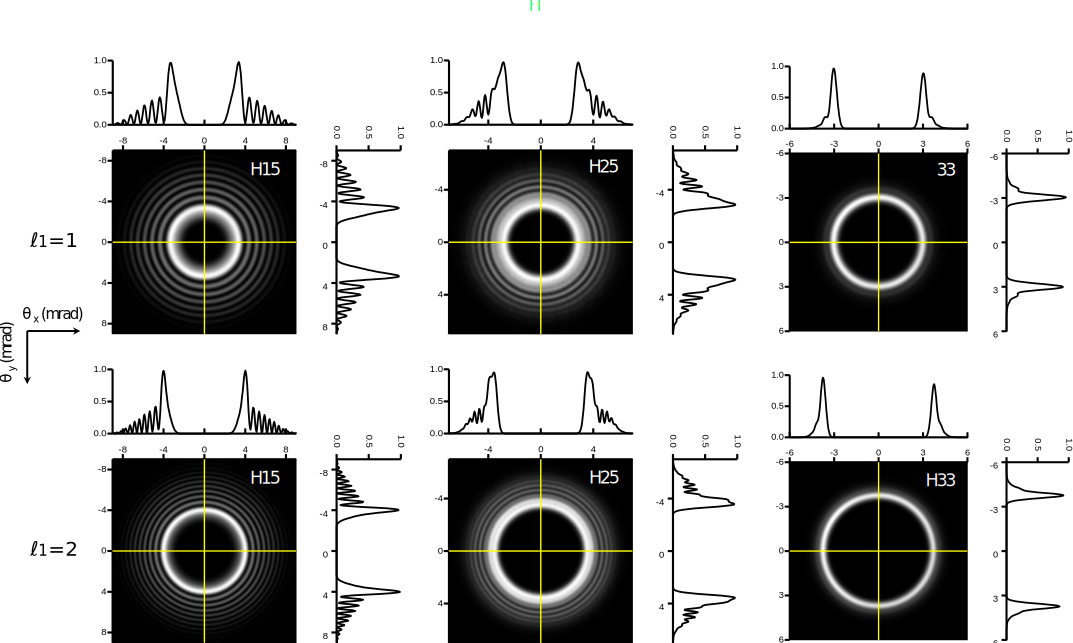
\includegraphics[width=\columnwidth]{Figures/Simul_LG_TA/FarFieldProfiles}%
\caption{Profil transverse d'intensité des harmoniques 15, 25 et 33 propagé 80 cm après le milieu de génération. Le laser infrarouge porte respectivement $\ell_1=1$ et 2 sur la ligne du haut et du bas. Des coupes des profils sont réalisées selon les lignes jaunes.}%
\label{Fig:FarFieldSimu}%
\end{figure}


Contrairement aux profils expérimentaux, ces images présentent une série d'anneaux concentriques autour d'un anneau central. Comme on le montrera, l'anneau le plus intense et central est généré par la trajectoire courte de la GHOE, tandis que les anneaux supplémentaires sont dus à la trajectoire longue. Dans l'expérience, on ne détecte que la contribution de la trajectoire courte, les conditions d'accord de phase étant apparemment défavorables à la génération de la longue. La figure \ref{Fig:DiamSimu} présente l'évolution du diamètre des anneaux, paramètre identifié comme central.

\begin{figure}[!ht]
\centering
\def\svgwidth{.9\columnwidth}
\import{Figures/Simul_LG_TA/}{diameter_simu.pdf_tex}
\caption{Diamètre des anneaux harmonique en champ lointain pour $\ell_1=1$ (cercles rouges) et $\ell_1=2$ (triangles bleus).}
\label{Fig:DiamSimu}
\end{figure}

Comme attendu, le diamètre est relativement constant sur tout le spectre, mis à part un saut vers l'harmonique 27. Ceci coïncide avec le domaine où les deux trajectoires quantiques commencent à fusionner : l'énergie de coupure est attendue à $I_c=I_p+3.14U_p=28.3\times(\hbar\omega_{IR})$. Dans cette zone, les trajectoires peuvent interférer spatialement et modulent le profil spatial des harmoniques. Le saut est alors interprété comme le passage d'une frange d'interférence sur l'anneau central. Cet effet est bien connu dans la GHOE par faisceau Gaussien \mycite{ZairPRL2008}.\par
Lorsqu'on double le MAO du faisceau de génération, le diamètre des harmoniques augmente de $1.4\approx\sqrt{2}$, ce qui est consistant avec la loi en $\sqrt{\ell_1}$ trouvée plus haut (\ref{eq:rmax_conservation}). 

\chapter{Le profil spatio-temporel des impulsions générées : les \textit{light springs}}
Jusqu'à présent nous nous sommes intéressés au moment angulaire orbital du faisceau et donc à ses propriétés spatiales. Une des propriétés remarquables de la GHOE est qu'elle permet de générer des impulsions extrêmement courtes, le record actuel étant de $\SI{67e-18}{s}=\SI{67}{as}$ (attosecondes). Dans cette partie nous étudions les propriétés temporelles des impulsions générées par un faisceau de LG, obtenues lorsqu'on considère la totalité du spectre harmonique.

\section{Mesure de la phase spectrale de l'impulsion à partir de la technique RABBIT}
\label{sec:omabbit}
Pour obtenir des informations temporelles, on cherche à mesurer à la fois l'intensité et la phase spectrale de l'impulsion. Nous disposons déjà de l'intensité spectrale, mesurée optiquement à l'aide du spectromètre. Pour la phase spectrale, nous choisissons d'appliquer la technique appelée RABBIT (\textit{Reconstruction of Attosecond Beating By
Interference of Two-photon Transitions}, reconstruction de battement attoseconde par
interférence de transitions à deux photons)

L'idée de cette technique est similaire à celle du SPIDER, dans laquelle on fait interférer différentes composantes spectrales du champ à caractériser. Dans ces interférences, on retrouve alors la différence de phase entre les différentes composantes fréquentielles. En pratique, on crée une réplique du faisceau décalée spectralement, et on fait varier le délai entre les deux répliques. \par Dans l'XUV, il est très difficile de créer une réplique du faisceau et de la décaler spectralement. Dans la technique RABBIT \mycite{MullerAPB2002}, ceci est réalisé à l'aide de la photoionisation d'un atome. La photoionisation crée un paquet d'onde électronique dont le spectre reflète celui des harmoniques du rayonnement utilisé (pics bleus de la figure \ref{fig:rabbit}. Pour faire interférer ces différents pics, on ajoute un champ infrarouge, dit d'habillage, qui rend possible de nouvelles transitions de photoionisation. Ce sont des transitions à deux photons et deux couleurs : absorption simultanée d'un photon harmonique et d'un photon infrarouge, et
absorption d'un photon harmonique et émission simultanée d'un photon infrarouge. Dans le spectre des photoélectron, on voit apparaître des pics satellites (\textit{sidebands}) situés entre les harmoniques (pics oranges sur la figure \ref{fig:rabbit}). Si le faisceau d'habillage a la même fréquence que celui de génération, ces pics sont équidistants des harmoniques adjacentes. 

\begin{figure}[!ht]
\centering
\def\svgwidth{1\columnwidth}
\import{Figures/RABBIT/}{rabbit_total.pdf_tex}
\caption{Principe de la technique RABBIT : le champ XUV est focalisé dans un jet de gaz, dont on collecte les photoélectrons. Le spectre des photoélectrons est une réplique du spectre harmonique (courbes bleues). Si on ajoute un faisceau d'habillage, on voit apparaître des pics satellites (courbes oranges).}
\label{fig:rabbit}
\end{figure}

On remarque que chaque pic satellite est issu de deux chemins quantiques différents : si son énergie est de $n+1$ unités de photons, il provient à la fois de l'absorption de $H_{n}$ et d'un photon infrarouge, et de l'absorption de $H_{n+2}$ et de l'émission d'un photon infrarouge. On scanne ensuite le délai entre les impulsions de génération et d'habillage, ce qui module l'intensité des pics satellites : les deux chemins quantiques interfèrent. Dans cette interférence, on mesure la phase spectrale relative entre les harmoniques $H_{n}$ et $H_{n+2}$.

Le dispositif expérimental utilisé est similaire à celui décrit par \mycite{MairesseScience2003} et utilisé à de maintes reprises par la suite \mycite{BoutuNP2008, DivekiNJP2012, HaesslerNJP2013, DivekiCP2013}. Pour effectuer une mesure RABBIT, le faisceau laser est séparé en deux parties dans un interféromètre de Mach-Zender, où la séparation et la recombinaison sont effectuées par des miroirs troués. Le délai entre les deux bras est contrôlé par une ligne à retard piézoélectrique de précision attoseconde. La partie centrale sert de faisceau d'habillage tandis que la partie annulaire est utilisée comme faisceau de génération : au foyer, ce faisceau annulaire présente un profil d'Airy dont le lobe central génère des harmoniques qui seront émises sur l'axe \mycite{PeatrossOL1994}. En champ lointain, le faisceau redevient annulaire et est donc spatialement séparé des harmoniques et du faisceau d'habillage. Ainsi, un simple iris permet de filtrer l'infrarouge de génération pour ne garder que le rayonnement harmonique et l'infrarouge d'habillage. Ces deux rayonnements sont focalisés par le miroir torique (voir figure \ref{Fig:ExpG}) au foyer duquel on place un spectromètre à temps de vol d'électrons à bouteille magnétique (TOF pour \textit{Time Of Flight}). Dans ce spectromètre, des photoélectrons sont créés par le rayonnement harmonique dans un second jet de gaz d'argon. Un électroaimant à pièces polaires trouées impose un champ magnétique initial d’environ 1 Tesla à l’endroit de la photoionisation, guidant les électrons vers un tube à temps de vol. Une fois collectés, les électrons sont guidés dans un champ magnétique faible sur une longueur d’1 m jusqu'à des galettes de micro-canaux. Les temps d’arrivée sur le détecteur sont discrétisés avec un pas d’une nanoseconde. Ce détecteur procure une résolution de 100 meV pour les électrons lents. 

Ici, le faisceau de génération et ses différentes harmoniques sont des modes de Laguerre-Gauss. Commençons par vérifier qu'après réflexion sur un miroir troué, le mode de LG n'est pas perturbé. On image simplement le foyer de la lentille de génération :
%
\begin{figure}[!ht]
\centering
\def\svgwidth{.7\columnwidth}
\import{Figures/OMABBIT/}{2Focus.pdf_tex}
\caption{Intensité de l'infrarouge au foyer de la lentille de génération, avec (droite) ou sans (gauche) réflexion sur un miroir troué.}
\label{Fig:2focus}
\end{figure}

Le foyer est donc une convolution entre une fonction d'Airy et le foyer sans miroir troué. Encore une fois, les rebonds extérieurs ne modifieront aucunement la GHOE; le miroir troué ne pose donc d'autre problème que de diminuer l'énergie disponible.
La deuxième question est celle de la photoionisation du gaz de détection par des faisceaux portant du MAO. Les conditions de focalisation étant douces ($f/\#\simeq 20/1$), l'approximation paraxiale est tout à fait vérifiée. Par conséquent, comme montré dans la partie \ref{sec:selectionrules}, les règles de sélection ne sont pas du tout modifiées par la présence de MAO : au niveau microscopique, la théorie habituelle du RABBIT s'applique. Au niveau macroscopique, le gaz d'atomes forme un volume fin selon la dimension longitudinale et plus grand que le faisceau dans la dimension transverse. Ainsi, le signal mesuré sur un pic satellite est une moyenne spatiale des contributions de chaque électron émis dans la région d'interaction. Considérons la composante oscillante du pic satellite $q+1$ en fonction du retard génération-habillage $\tau$. Un point $(r,\theta)$ dans la région d'interaction y contribue selon la loi suivante \mycite{VeniardPRA1996} : 
\begin{align*}
  & \text{S}{{\text{B}}_{q+1}}\left( \tau ,r,\theta  \right)=\text{cos}\left[ 2\omega {\left(\tau-{\tau }_{0}\right)}+{{\varphi }_{q+2}}-{{\varphi }_{q}}+{{\Phi }_{q+2}}\left( r,\theta  \right)-{{\Phi }_{q}}\left( r,\theta  \right)-2{{\Phi }_{hab}}(r,\theta ) \right],
\end{align*}
où on a négligé les phases atomiques et où on a noté $\omega$ la pulsation de l'infrarouge, $\tau_0$ l'origine des temps, $\varphi_q$ et $\Phi_q(r,\theta)$ les phases spectrales et spatiales de l'harmonique $q$, et ${\Phi }_{hab}(r,\theta)$ la phase spatiale du faisceau d'habillage. Pour les harmoniques, $\Phi_q(r,\theta)=\ell_q\theta = q\times\ell_1\theta$. Le signal intégré sur le volume de photoionisation est donc donné par :
\begin{equation*}
\text{S}{{\text{B}}_{q+1}}\left(\tau\right)=\iint_{r,\theta}{\text{cos}\left[ 2\omega {\left(\tau-{\tau }_{0}\right)}+{{\varphi }_{q+2}}-{{\varphi }_{q}}+\left(\ell_{q+2}-\ell_q\right)\theta-2{{\Phi }_{hab}}(r,\theta ) \right]r\rmd r \rmd \theta}.
\end{equation*}
Si $\left(\ell_{q+2}-\ell_q\right)\theta-2{{\Phi }_{hab}}(r,\theta ) =0 $, alors l'intégration selon $\theta$ du cosinus donne un résultat non nul. On obtient donc une condition suffisante pour observer une trace RABBIT : 
\begin{equation*}
{\Phi }_{hab}(r,\theta )=\left(\ell_{q+2}-\ell_q\right)\theta/2=\ell_1\theta,
\end{equation*}
c'est-à-dire que le faisceau d'habillage porte le même MAO que le faisceau de génération. Expérimentalement, on déplace simplement le masque de phase en spirale en amont de l'interféromètre de Mach-Zender. Notons pour finir qu'on peut effectuer le raisonnement dans l'autre sens : si on ne connaît pas le MAO harmonique $\ell_q$, et qu'on observe des sidebands oscillantes avec ${\Phi }_{hab}(r,\theta )=\ell_1\theta$, alors $\left(\ell_{q+2}-\ell_q\right)=2\ell_1\theta$. L'observation d'oscillations est alors vue comme une preuve que le rayonnement harmonique est bien accordé sur le faisceau d'habillage connu. Nous avons essayé de pousser ce raisonnement pour effectuer des mesures RABBIT résolues spatialement pour un faisceau quelconque en modulant le faisceau d'habillage. Ce fut le sujet d'une campagne d'expériences dans le groupe du professeur L. DiMauro à Columbus, Ohio qui n'a pour l'instant pas été conclue.

Avec le faisceau d'habillage adéquat, nous avons pu mesurer la trace RABBIT présentée sur la figure \ref{Fig:omabbit} quand les deux faisceaux infrarouges portaient $\ell_1=1$.

\begin{figure}[!ht]
\centering
\def\svgwidth{\columnwidth}
\import{Figures/OMABBIT/}{rabbit_trace.pdf_tex}
\caption{Trace RABBIT avec faisceau portant du MAO. (a) Spectrogramme de la photoionisation à deux couleurs et à deux photons de l'argon, le champ générateur portant $\ell_1=1$. Les lignes brillantes correspondent aux harmoniques impaires, tandis que les lignes plus faibles et oscillantes, de périodicité T=2.66 fs et 1.33 fs, sont les sidebands. (b) Spectre moyenné sur le retard en échelle logarithmique (rouge) et délai de groupe de l'impulsion attoseconde (cercles bleus, la surface bleue claire représentant la barre d'erreur d'analyse numérique à $3\sigma$).}
\label{Fig:omabbit}
\end{figure}

On observe clairement des pics satellites oscillant à $2\omega$ (période de  $\SI{1.33}{fs}$). Elles présentent également une autre composante à $\omega$, effet inévitable dans notre schéma. En effet, le faisceau d'habillage se propage à travers le milieu de génération et module le rendement de génération harmonique à la fréquence $\omega$. Comme expliqué, la présence d'oscillations à $2\omega$ confirme une fois de plus la conservation du moment angulaire orbital dans le processus. On cherche ensuite la phase de l'oscillation à $2\omega$, et on obtient le délai de groupe présenté en \ref{Fig:omabbit}~(b) : il s'agit de la dérivée de la phase spectrale de l'impulsion attoseconde. Un fit linéaire de cette courbe donne une pente de $103\pm9$ as, ce qui est exactement la même valeur que celle obtenue avec un faisceau Gaussien à la même longueur d'onde et à la même intensité de génération \mycite{MairesseScience2003}. Les processus de GHOE et de photoionisation n'étant pas changés à l'échelle microscopique, le MAO ne peut pas modifier les phases induites par ces processus, ce qui explique qu'on retrouve la même valeur.

\section{Reconstruction du profil spatio-temporel de l'émission}
Nous disposons désormais d'informations d'intensité et de phase spatiales et spectrales, à partir desquels on va reconstruire le profil spatio-temporel de l'émission attoseconde. Nos impulsions infrarouges de 50 fs comportent de nombreux cycles, on néglige donc les effets d'enveloppe et on écrit en $z = 0$ :
\begin{equation*}
I_{atto}(r,\theta,t) = \sum_{q=11}^{23}\;\sqrt{I_q(r,\theta)}\cdot\exp{(\rmi\left[\Phi_q(r,\theta)+\phi_q+\omega_q t\right])}.
\end{equation*}
On effectue alors l'hypothèse, justifiée dans la partie \ref{sec:oam_cons}, que la phase spatiale des harmoniques $\Phi_q(r,\theta)$ est celle d'un mode de Laguerre-Gauss parfait : $\Phi_q(r,\theta) = \ell_q \theta$. La phase spectrale $\phi_q$ est donnée par la mesure RABBIT, tandis que l'intensité $I_q(r,\theta)$ est donné par la mesure optique. On obtient alors l'isosurface d'intensité représentée sur la figure \ref{Fig:corkscrew}.

\begin{figure}[!ht]
\centering
\def\svgwidth{\columnwidth}
\import{Figures/OMABBIT/}{corkscrew.pdf_tex}
\caption{Profil spatio-temporel de l'émission. (a) Iso-surface d'intensité de l'impulsion attoseconde à 80\% de sa valeur maximale. Le panneau noir et blanc est une projection de cette intensité dans le plan $t=-2$ fs. (b) Coupes temporelles pour trois différents angles dans l'impulsion attoseconde $\theta=0$\degres (rouge), $\theta=40$\degres (bleu pointillé) et $\theta=-60$\degres (vert).}
\label{Fig:corkscrew}
\end{figure}

On observe une structure en tire-bouchon, déjà prédite théoriquement par \mycite{HernandezPRL2013} puis décrite par \mycite{ParienteOL2015}, qui l'ont nommée \textit{light springs} (ressort optique en français). Ici, on trouve deux ressorts entrelacés, conséquence de la présence des harmoniques impaires seulement. En effet, dans un plan $t$ donné, on somme plusieurs harmoniques séparées de $\Delta\ell = 2$. Une périodicité doublée dans un espace impose une périodicité de moitié dans l'espace réciproque, donc $\Delta\theta = \pi$ : on trouve bien deux lobes d'intensité dans chaque plan $t$ donné. Le profil temporel quant à lui possède bien une structure de train d'impulsions attoseconde, où chaque impulsion dure environ 200 as. Cette structure présente un couplage spatio-temporel particulièrement intéressant : comme illustré sur la droite de la figure \ref{Fig:corkscrew}, si on change l'angle auquel on regarde le train d'impulsions, on observe le même train, mais retardé. Par exemple, entre $\theta=0$\degres et $\theta=40$\degres, on obtient un retard de 296 as. En 180$\degres$, on effectue une demi-période du laser infrarouge de génération (1330 as), la pente est donc de 7.4 as/\degres. 
Comme démontré dans \mycite{HernandezPRL2013}, la structure de light spring existe toujours dans le cas d'une impulsion attoseconde unique. Nous pensons donc que ce type d'impulsion constitue une sonde particulièrement pratique pour des expériences de spectroscopie d'absorption transitoires : en effet, ces expériences nécessitent de réaliser et de contrôler des retards pompe-sonde de l'ordre de l'attoseconde. Ici, on peut paramétrer le délai attoseconde sur la coordonnée angulaire en un seul tir laser, rendant l'expérience insensible aux instabilités. Dans une expérience pompe-sonde, l'autre paramètre est la gamme dynamique : elle est ici de 1.33 fs, i.e. le demi-cycle optique infrarouge. Cette gamme peut être facilement augmentée en augmentant la longueur d'onde de génération ou encore en brisant la symétrie du processus, de sorte à générer des harmoniques paires.

\chapter{Contrôle du nombre quantique radial par la sélection de trajectoires quantiques}
\label{sec:pmodes}
\section{Rôle de la phase atomique dans la génération de modes de nombre radial non nul}
\`{A} la partie \ref{sec:sfa}, nous avons effectué des simulations numériques quantiques (SFA). Nous avons déjà vu que les profils obtenus en champ lointain montrent deux contributions distinctes, que nous avons attribué aux deux premières trajectoires quantiques de la GHOE. Pour étudier ce point plus en détail, on peut varier la position $z_0$ du foyer infrarouge par rapport au jet de gaz, qui contrôle le poids relatif des trajectoires. Pour la figure \ref{Fig:FarFieldSimu}, nous avions $z_0=0$. La figure \ref{Fig:H21_traj}~(a-c) présente le profil obtenu en champ lointain lorsque le laser est focalisé en amont, au milieu, et en aval du jet. Quand $z_0<0$, c'est-à-dire que le laser est focalisé avant le jet, l'accord de phase favorise fortement la trajectoire courte. Dans ce cas, le profil en champ lointain ne présente qu'un seul anneau : comme dans l'expérience on génère un mode de Laguerre-Gauss quasiment pur. Au contraire si $z_0>0$, on observe plusieurs anneaux sur un profil qui rappelle un mode de LG avec $p\neq 0$. Dans le cas intermédiaire, le profil est beaucoup plus modulé à cause des interférences entre trajectoires quantiques. On vérifie cet effet en sélectionnant numériquement tour à tour une seule trajectoire. Les panneaux \ref{Fig:H21_traj}~(d,e) montrent que l'on retrouve bien un anneau presque pur pour la courte, et une série d'anneaux pour la longue.

\begin{figure}[!ht]
\centering
\def\svgwidth{.7\columnwidth}
\import{Figures/Simul_LG_TA/}{trajectories.pdf_tex}
\caption{Contributions des différentes trajectoires quantiques dans la GHOE par faisceau LG. Le profil d'intensité de l'harmonique 21 est présenté pour (a) $z_0<0$, (b) $z_0=0$, (c) $z_0>0$. La convention de signe est illustrée au-dessus. Les profils (d) et (e) sont calculés avec $z_0=0$ en ne prenant en compte que la contribution respectivement de la trajectoire courte ou longue.}
\label{Fig:H21_traj}
\end{figure}

\section{Observation de modes de nombre quantique radial élevé}
\subsection{Modification du dispositif expérimental}
Cherchons maintenant à observer des profils similaires de manière expérimentale. On s'attend à observer l'apparition d'anneaux supplémentaires plus divergents et moins intenses, il faut adapter notre dispositif en conséquence. En particulier, le réseau cylindrique de diffraction risque de distordre l'image trop fortement, nous avons donc cherché à construire un spectromètre donnant véritablement une image en coordonnées ``spatiale-spatiale''. 
Nous avons repris le schéma proposé par Hartmut Ruf dans sa thèse \mycite{Ruf2012}. L'idée est d'illuminer aussi peu de traits du réseau que possible, de sorte à réduire la dispersion induite par le réseau. De plus, on cherche à utiliser un dispositif le moins astigmate possible, de sorte à éviter les effets de conversion $\mathcal{LG}\rightarrow \mathcal{HG}$. Pour ce faire, on utilise un réseau de diffraction en incidence quasi-normale. Pour réduire le nombre de traits illuminés, le faisceau est d'abord focalisé par un miroir sphérique, lui aussi en incidence quasi-normale. Le réseau est alors positionné juste avant le foyer du miroir de sorte à rester en dessous du seuil de dommage. Bien sûr, l'incidence normale des optiques réduit fortement le flux dans l'UVX. Pour garantir une réflectivité correcte, le miroir sphérique est traité avec un revêtement de $\mathrm{B}_\mathrm{4}\mathrm{C}$, qui réfléchit à 10-30 \% jusqu'à l'ordre harmonique 19 avec un angle d'incidence de 10$\degres$ (voir figure \ref{Fig:reflectivity_B4C}). 

\begin{figure}[!ht]
\centering
\def\svgwidth{.6\columnwidth}
\import{Figures/Hartmut_Spectro/}{reflectivity_b4c.pdf_tex}
\caption{Réflectivité mesurée du miroir avec revêtement de $\mathrm{B}_\mathrm{4}\mathrm{C}$ en fonction de la longueur d'onde. L'angle d'incidence est de 10$\degres$. Adapté de \mycite{Ruf2012}.}
\label{Fig:reflectivity_B4C}
\end{figure}

Le réseau de diffraction (Spectrogron) dispose de $\sigma=\SI{600}{grooves/mm}$, son principal avantage étant son faible coût (600€), à comparer avec le prix des réseau cylindriques habituels (de l'ordre de 10000€). Le dispositif complet est présenté sur la figure \ref{Fig:DispHartmut}. Ce dispositif nous a été prêté par nos collègues du CELIA Bordeaux, Yann Mairesse et Valérie Blanchet. L'utilisation de ce spectromètre, outre sa transmission relativement faible, présente deux difficultés. Tout d'abord, en champ intermédiaire, avec nos sources relativement étendues, nous observons une superposition d'anneaux. Il faut donc placer une fente de sortie au foyer et balayer le spectre avec cette fente, afin de ne sélectionner qu'une harmonique. Le deuxième point délicat est la calibration du spectromètre : il est a priori difficile de distinguer les différents ordres de diffraction entre eux. 

\begin{figure}[!ht]
\centering
\def\svgwidth{\columnwidth}
\import{Figures/Hartmut_Spectro/}{disp_exp.pdf_tex}
\caption{Dispositif expérimental avec spectromètre peu dispersif. Le faisceau infrarouge est mis en forme par une lame de phase en spirale (SPP) et focalisé par une lentille (L) de longueur focale $f=1m$. Les harmoniques du fondamental sont générées dans le jet de gaz d'argon et réimagées par un ensemble miroir torique (MT) + lame de silice (LS). Le spectromètre est constitué d'un miroir sphérique recouvert de $\mathrm{B}_\mathrm{4}\mathrm{C}$ à 10$\degres$ d'incidence et d'un réseau de diffraction à $\approx 6\degres$ d'incidence. Au foyer, on place une fente permettant de sélectionner une unique harmonique, qui est ensuite imagée par l'ensemble MCP+écran de phosphore.}
\label{Fig:DispHartmut}
\end{figure}

\subsection{Calibration du spectromètre}
\label{sec:calib}
Pour calibrer le spectre, il faut pouvoir reconnaître plusieurs ordres de diffraction correspondant à la même longueur d'onde. Pour ce faire, nous choisissons d'utiliser une technique d'interférométrie à deux faisceaux, similaire à celle proposée par \mycite{bertrandprl2011}. \`{A} l'aide d'un interféromètre, on rajoute un deuxième faisceau de perturbation à 800nm, non-colinéaire au premier. Au foyer, les deux faisceaux se croisent avec un angle et créent un réseau de diffraction dans la dimension verticale. Ainsi, il est possible d'absorber un photon venant du deuxième faisceau comme schématisé sur la figure \ref{Fig:DiffSchema}. On observe donc deux pics venant de deux chemins quantiques différents : par exemple pour l'harmonique 11, on peut absorber 11 photons du faisceau principal et créer le pic habituel, ou bien absorber 10 photons du principal et 1 de la perturbation. La conservation des moments nous donne la position de ce nouveau pic, qui est diffracté dans la dimension verticale. Comme sa position dépend de la longueur d'onde de l'harmonique mais pas de l'ordre de diffraction du réseau, la distance entre pic principal et diffracté permet d'identifier 
les différents ordres de diffraction du réseau de diffraction. Notons qu'en pratique, on a des chemins quantiques d'ordre supérieur, ce qui amène à la génération de pics supplémentaires, éventuellement diffractés de l'autre côté du pic principal.

\begin{figure}[!ht]
\centering
\def\svgwidth{\columnwidth}
\import{Figures/Hartmut_Spectro/}{schema_2beam.pdf_tex}
\caption{Schéma de l'expérience de calibration à deux faisceau pour l'harmonique 11. Le faisceau principal (rouge) est plus intense que le faisceau de perturbation (orange). Ainsi, on a un pic central dominant dans lequel on a absorbé 11 photons de la génération, et un pic diffracté où on a absorbé un photon de la perturbation. La conservation des moments donne directement la direction d'émission de l'harmonique diffractée.}
\label{Fig:DiffSchema}
\end{figure}

Le réseau de diffraction est monté sur une rotation motorisée de sorte à pouvoir balayer l'angle de réflexion. La figure \ref{Fig:calibration} montre les profils obtenus pour différents angles du réseau. On distingue clairement un ou plusieurs ordres de diffraction à côté d'un pic principal. Il reste à mesurer la distance entre les deux pics et à les tracer pour chacune des harmoniques, comme fait en bas de la figure \ref{Fig:calibration}. On notera que l'axe horizontal n'est pas l'angle de réflexion de chaque harmonique, les harmoniques n'ayant pas été imagées une par une. La mesure n'est pas extrêmement précise du fait des inhomogénéités des profils mais on trouve quand même 6 uniques valeurs d'écart entre les pics, à $\pm 2$ pixel près. On détecte donc 6 harmoniques différentes. Ces valeurs reviennent 2 à 3 fois, ce qui signifie que l'on mesure jusqu'à l'ordre 3 du réseau de diffraction. La distance entre les pics diminue avec l'ordre harmonique, ce qu'on retrouverait en traçant l'image photonique de la figure \ref{Fig:DiffSchema} pour chaque harmonique.

\begin{figure}[!ht]
\centering
\def\svgwidth{\columnwidth}
\import{Figures/Hartmut_Spectro/}{calibration_v2.pdf_tex}
\caption{Calibration du spectromètre. Un second faisceau infrarouge vient perturber la génération et créer un pic satellite, dont la position dépend de la longueur d'onde. En haut, profil spatial des harmoniques détectées pour différents angles du réseau. En bas, les points rouges représentent la distance entre les deux pics pour les harmoniques correspondantes.\`{A} $\pm2$ pixel près, on retrouve 6 valeurs qui permettent d'identifier 6 harmoniques (rectangles colorés). Les traits noirs relient les ordres de diffraction du réseau. L'identification des ordres harmoniques est expliquée plus bas.}
\label{Fig:calibration}
\end{figure}

Il reste à identifier quelles sont les 6 harmoniques observées. Pour ce faire, on utilise la formule des réseaux :
\[\sin(\theta_r^q)+\sin(\theta_i) = \frac{m\lambda_q}{d},\]
où $\theta_r^q$ et $\theta_i$ sont les angles de réflexion et d'incidence, $m$ est l'ordre de diffraction et $d$ est le pas du réseau. La valeur de $d$ donnée par le fournisseur est $1/600\simeq \SI{1.67}{\micro \metre}$. La figure \ref{fig:formulereseau} trace l'évolution de $\theta_r^q$ pour les harmoniques 9 à 19 (celles plus élevées sont absorbées par le $\mathrm{B}_\mathrm{4}\mathrm{C}$, voir figure \ref{Fig:reflectivity_B4C}) pour des valeurs de $d$ autour de $\SI{1.67}{\micro\metre}$. Les deux premiers ordres de diffraction sont représentés. On cherche une harmonique singulière qui pourrait être identifiée dans l'expérience. On remarque que l'harmonique 9 de l'ordre 1 est située entre les harmoniques 17 et 19 de l'ordre 2. C'est le seul recouvrement entre les deux premiers ordres de diffraction. L'harmonique 9 est donc facilement identifiable sur la figure \ref{Fig:calibration}, où elle est pointée par une flèche rouge.

\begin{figure}[!ht]
\centering
\def\svgwidth{1\columnwidth}
\import{Figures/Hartmut_Spectro/}{Diffraction_f_d.pdf_tex}
\caption{Angle de réflexion des harmoniques 9 à 19 en fonction du pas du réseau de diffraction. Les ordres de diffraction 1 et 2 sont représentés.}
\label{fig:formulereseau}
\end{figure}

\subsection{Résultats}
Le spectre étant maintenant calibré, on procède à des mesures de spectres harmoniques. Comme dans les calculs numériques, on varie $z_0$ pour changer le poids relatif des trajectoires quantiques. La figure \ref{Fig:LensScan} présente l'évolution du profil des cinq premières harmoniques lorsqu'on balaye $z_0$ sur 1.2 cm. Notons que la définition de $z_0=0$ est ici presque arbitraire : il est très difficile de connaître expérimentalement la véritable valeur de $z_0$, on ne peut donc que définir $z_0=0$ pour reproduire la simulation (figure \ref{Fig:H21_traj}).

On observe des séries d'anneaux très symétriques et assez homogènes, signe que l'on observe bien le profil ``spatial-spatial'' des harmoniques, et non pas une convolution spatio-spectrale. Pour $z_0=-0.2$ cm, on observe un unique anneau, mis à part pour l'harmonique 9 où un second anneau est imbriqué. Ce second anneau est probablement dû à une mauvaise sélection par la fente, qui laisse passer une harmonique diffractée au deuxième ordre par le réseau, le deuxième ordre étant particulièrement proche du premier dans cette région (voir figure \ref{Fig:calibration}. Pour $z_0=0$ cm, on voit apparaître un nouvel anneau au centre de l'image. Les calculs théoriques (figure \ref{Fig:H21_traj}) montrent un effet similaire à $z_0=0$, que nous avons interprété comme une interférence entre les deux trajectoires quantiques. C'est cette particularité nous a amené à définir $z_0=0$ à cet endroit. Ensuite, à mesure que $z_0$ augmente, on voit apparaître un nombre croissant d'anneaux concentriques plus divergents, en accord la théorie. Ces anneaux sont dues à la trajectoire longue de la GHOE. Ils suggèrent la génération de modes de LG de mode $p\neq 0$. Nous allons vérifier ce point en cherchant où ces modes peuvent être produits dans la GHOE.


\begin{figure}[!ht]
\centering
\def\svgwidth{1\columnwidth}
\import{Figures/P_Modes/}{results_pmodes.pdf_tex}
\caption{Profil d'intensité des harmoniques 9 à 17 (axe horizontal) lorsque la lentille de génération est déplacée sur 1.2 cm (axe vertical). Chaque harmonique est normalisée à 1.}
\label{Fig:LensScan}
\end{figure}

\clearpage
\section{Interprétation des résultats : le rôle de l'indice radial des modes de Laguerre-Gauss}
Rappelons l'expression du champ d'un mode de Laguerre-Gauss d'incice $(\ell,p)$ :

\begin{align}
{E_{\ell,p} }\left( {r,\theta ,z} \right) &= {\;}\frac{C_{\ell,p}}{w(z)}
{\left( {\frac{r\sqrt{2}}{{w\left(z\right)}}} \right)^{\left| \ell  \right|}}
\exp{\left(- \frac{{{r^2}}}{{{{w^2(z)}}}}\right)}
L_p^{\left| \ell  \right|}\left(\frac{2r^2}{w^2(z)}\right)\nonumber\\
&\times
\exp{({\rmi}\ell \theta )}
\exp{\left(-{\rmi}k\frac{r^2}{2R(z)}\right)}
\exp{(-{\rmi}kz)}
\exp{(\rmi(2p+\left|\ell\right|+1)\chi(z))},
\label{eq:lgmodes2}
\end{align} 

\subsection{Sens physique de l'indice radial}
Comme mentionné plus haut, le profil obtenu quand la trajectoire longue domine ressemble à un mode de Laguerre-Gauss de $p\neq 0$. Il est a priori impossible de connaître le contenu modal exact à partir d'une mesure d'intensité : le mode peut être une superposition d'un grand nombre de modes de $p$ différents, ayant chacun une phase et une amplitude inconnues. On peut toutefois chercher d'où ces modes $p$ proviennent dans l'expérience réalisée.

N'étant pas relié à la grandeur physique du MAO, le sujet de l'indice radial des modes de Laguerre-Gauss a longtemps été délaissé. En général, la présence de modes $p\neq 0$ est indésirable et considérée comme du bruit dans la génération d'un mode $(\ell,p=0)$ pur. C'est seulement assez récemment que des équipes se sont intéressées à ce paramètre, le nommant par exemple \textit{the forgotten quantum number} \mycite{Plickpra2015}. \mycite{KarimiPRA2014} ont réalisés des interférences de Hong-Ou-Mandel, montrant que $p$ était un nombre quantique valable. L'indice $p$ a été utilisé par \mycite{SalakhutdinovPRL2012} et \mycite{KrennPNAS2014} pour produire des états intriqués de dimensions impressionantes, et ses propriétés physiques sont étudiées en détail dans \mycite{Plickpra2015} et 	\mycite{KarimiPRA2014-2}. Enfin, \mycite{MendozaOL2015} ont montré que les modes de $p$ élevés avaient des propriétés d'auto-régénération similaires à celles d'un faisceau de Bessel. L'auto-régénération signifie que si même si une partie du faisceau est obstruée, le mode se reconstitue au cours de sa propagation, propriété très intéressante pour le transmission d'information.

Il est donc intéressant de chercher à produire et à contrôler les modes $p$ dans l'extrême ultra-violet, au lieu de les voir comme un effet parasite. Pour créer des modes $p\neq 0$, on pourrait modifier directement le mode infrarouge. Cependant, dû à la forte non-linéarité de la GHOE, il est probable que les anneaux extérieurs ne contribuent pas à la génération. Une autre approche est de chercher dans le processus de GHOE lui-même, une variable permettant d'augmenter le mode radial. Comme dit plus haut, $p$ est un nombre quantique, valeur propre d'un opérateur qui vérifie $\hat{N}\ket{\mathcal{LG}_{(\ell,p)}(r,\theta,z)} = p\ket{\mathcal{LG}_{(\ell,p)}(r,\theta,z)}$. L'expression de cet opérateur est donnée par \mycite{Plickpra2015} et \mycite{KarimiOL2012}. On sait que le moment linéaire est relié à la translation, le moment angulaire à la rotation, et ces travaux démontrent que $p$ est lui relié à la \textit{dilatation} selon la coordonnée radiale. Tout effet créant une forme de dilatation radiale du faisceau modifiera donc le contenu en mode $p$ du champ.

Nous avons déjà vu qu'au foyer le faisceau infrarouge est bien décrit par un mode $\mathcal{LG}_{(\ell,p=0)}$ (voir section \ref{sec:spp}). Dans la GHOE, on identifie deux effets menant à une modification radiale du champ : 
\begin{enumerate}
\item La non-linéarité de la GHOE : si un processus a une non-linéarité d'ordre $n$, alors le champ obtenu sera $E_{out}=E_{in}^n$. Un profil Laguerre-Gaussien sera donc modifié en profil plus piqué autour de ses maxima.

\item La phase du moment dipolaire atomique : dans le modèle à trois étapes, l'électron acquiert une phase au cours de sa propagation qui dépend de l'intensité infrarouge locale. Le rayonnement émis présente donc une phase non uniforme spatialement. Dans le plateau, cette phase est approximativement linéaire avec l'intensité \mycite{SalieresPRL1995}. Elle s'écrit $\phi^{at}(r,\theta) = \alpha_{traj} I_{IR}(r,\theta)$, où $\alpha_{traj}$ est un coefficient de proportionnalité dépendant de la trajectoire quantique en question. Ici, $I_{IR}(r,\theta)$ est un mode de Laguerre-Gauss. Cette phase spatiale peut donc modifier le mode et créer une forme de dilatation.
\end{enumerate}
Nous allons étudier ces deux effets en effectuant des simulations numériques.

\subsection{\'{E}tude du contenu modal du champ par un modèle simple de la GHOE}
Pour étudier ces effets, une description simple du processus est suffisante. On ne prendra pas en compte les effets liés à la propagation du champ ni les effets de dispersion et de déplétion dans le milieu. On considère donc un plan d'atomes infiniment fin placé en $z=0$. On se place dans les conditions expérimentales pour calculer la propagation du champ infrarouge jusqu'au foyer, et on obtient le champ déjà présenté en figure \ref{Fig:DecompIR}. On utilise ensuite la formule ADK \mycite{AmmosovJETP1986} et le modèle SFA \mycite{LewensteinPRA1994} pour calculer le dipôle harmonique qui donne directement le champ émis. Les deux effets mentionnés plus haut sont alors simples à identifier : la non-linéarité est contrôlée par l'intensité du champ infrarouge, tandis que la phase atomique varie à la fois avec l'intensité et avec la valeur de $\alpha_{traj}$, qui dépend de la trajectoire considérée.

\paragraph*{Trajectoire courte} Commençons par sélectionner uniquement la trajectoire courte de la GHOE, ce qui est réalisé expérimentalement en choisissant la position du foyer en amont du jet. Pour cette trajectoire, $\alpha_{courte}$ est de l'ordre de $\SI{-1e-14}{cm²/W}$. Pour des intensités crêtes de l'ordre $\SI{1e14}{W/cm²}$, on aura un déphasage de l'ordre du radian entre le centre et le bord de l'anneau. C'est une courbure relativement faible. La figure \ref{Fig:DecompShort}~(a) présente le champ harmonique obtenu en $z=0$ pour l'harmonique 19.

On voit bien l'effet de $\phi^{at}$ sur la phase spatiale, avec une légère courbure le long de l'anneau. On effectue ensuite une décomposition en modes de Laguerre-Gauss de ce champ, grâce à la formule \ref{Eq:decompLG}, en choisissant $w_0 = r_{max}\sqrt{2/|\ell_q|}$ (équation \ref{Eq:rmax_LG}). Les résultats sont présentés sur le panneau (b) de la figure \ref{Fig:DecompShort}. Le champ est composé à 98,9\% du mode $(\ell,p) = (0,0)$. De manière surprenante, ce mode est encore plus pur que le champ infrarouge utilisé pour le générer. C'est un effet de la non-linéarité du processus, qui ne fait contribuer que les parties les plus intenses du faisceau infrarouge et gomme les reliquats dus au vignetage et aux imperfections de la lame de phase. En conclusion, on voit que l'effet (i) et l'effet (ii) avec une valeur faible de $\alpha_{traj}$ ne perturbent aucunement le contenu du mode et ne sont pas responsables des anneaux observés en champ lointain. On peut illustrer ce point en propageant numériquement ce champ jusqu'au détecteur, ce qui est montré sur la figure \ref{Fig:DecompShort}~(c). On observe bien un anneau unique.
\begin{figure}[!ht]
\centering
\def\svgwidth{\columnwidth}
\import{Figures/P_Modes/}{short_trajectory.pdf_tex}
\caption{Profil de l'harmonique 19 généré par la trajectoire courte. (a) Champ au foyer. De gauche à droite, intensité spatiale, phase spatiale, et représentation mixte où la couleur donne la phase et la luminosité l'intensité. (b) Module des coefficients de la décomposition du champ sur la base de Laguerre-Gauss. Les coefficients de module inférieur à $\num{1e-4}$ sont ignorés. (c) Intensité en fonction de $z$ obtenue par propagation du champ présenté en (a).}
\label{Fig:DecompShort}
\end{figure}

\paragraph*{Trajectoire longue} Effectuons maintenant le même calcul dans le cas de la trajectoire longue. La figure \ref{Fig:DecompLong} présente les résultats obtenus. Dans ce cas, $\alpha_{longue}\approx\SI{-20e-14}{cm²/W}$, valeur 20 fois plus élevée que pour la trajectoire courte. Comme on le voit sur la phase spatiale, la courbure de phase est ici beaucoup plus importante. Quand on effectue la décomposition sur la base de Laguerre-Gauss, on obtient une superposition d'un assez grand nombre de modes ayant $\ell_{19}=19$ et $p$ allant de 0 à $\approx 30$. Le mode $(0,0)$ domine toujours, mais ne compte que pour 52\% de l'émission\footnote{La figure \ref{Fig:DecompLong}~(b) donne les coefficients $\left|c_{\ell,p}\right|$. La normalisation du champ s'écrit $\sum_{\ell,p}{\left|c_{\ell,p}\right|^2} = 1$, c'est donc $\left|c_{\ell,p}\right|^2$ qui donne la contribution du mode $(\ell,p)$ en pourcentage.}. 

\begin{figure}[!ht]
\centering
\def\svgwidth{\columnwidth}
\import{Figures/P_Modes/}{long_trajectory.pdf_tex}
\caption{Profil de l'harmonique 19 généré par la trajectoire longue. (a) Champ au foyer. De gauche à droite, intensité spatiale, phase spatiale, et représentation mixte où la couleur donne la phase et la luminosité l'intensité. (b) Module des coefficients de la décomposition du champ sur la base de Laguerre-Gauss. Les coefficients de module inférieur à $\num{1e-4}$ sont ignorés. (c) Intensité en fonction de $z$ obtenue par propagation du champ présenté en (a).}
\label{Fig:DecompLong}
\end{figure}

Comme le montre le calcul de propagation, en champ lointain ces modes interfèrent et créent une série d'anneaux concentriques similaires à ceux observés expérimentalement. Au foyer, les coefficients des différents modes sont tels que l'intensité ne présente qu'un seul anneau. Puisqu'on a des modes, les coefficients de la décomposition ne changent pas au cours de la propagation, mais l'intensité est modifiée. Cela signifie que la phase relative entre les différents modes de Laguerre-Gauss évolue au cours de la propagation. En regardant l'expression des modes de Laguerre-Gauss (équation \ref{eq:lgmodes2}), on voit que le seul terme responsable est la phase de Gouy, qui s'écrit :
\begin{equation*}
\psi _{\ell ,p}(z)=(2p+\left|\ell\right|+1)\arctan{\frac{z}{z_R}}.
\end{equation*}
Pour $z\gg z_R$, le mode $(\ell,p)$ a donc acquis une phase $(2p+\left|\ell\right|+1)\frac{\pi}{2}$, soit une différence de $\pi$ avec les modes $p-1$ et $p+1$. 

En conclusion, nous avons relié la présence de modes $p$ dans la GHOE à la phase $\phi^{at}=\alpha_{traj} I_{IR}$. Cette phase dépend à la fois de la trajectoire considérée et de l'intensité infrarouge. L'intensité fournit donc un paramètre d'ajustement supplémentaire. La figure \ref{Fig:H19_Iscan} présente l'évolution du contenu modal pour chaque trajectoire, lorsque l'intensité infrarouge varie entre 1 et $\SI{2.4e14}{W/cm^2}$.

\begin{figure}[!ht]
\centering
\def\svgwidth{\columnwidth}
\import{Figures/P_Modes/}{H19_Iscan.pdf_tex}
\caption{\'Evolution du contenu modal avec l'intensité infrarouge pour les deux premières trajectoires quantiques.}
\label{Fig:H19_Iscan}
\end{figure}

Pour la trajectoire courte, l'intensité n'a aucune influence sur le contenu modal, à cause de la faible valeur de $\alpha_{traj}$. Au contraire, le nombre de modes constituant le champ émis par la trajectoire longue passe de $\simeq 8$ à plus de 30 sur cette gamme d'intensité. 

\chapternonum{Conclusion et perspectives de la partie II}
En conclusion, nous avons détaillé dans ce chapitre comment générer des harmoniques d'ordre élevé à partir d'un faisceau de Laguerre-Gauss. Nous avons mis en évidence les difficultés supplémentaires et les différences par rapport au cas Gaussien habituel. Grâce à des calculs numériques, nous avons démontré qu'une simple observation de l'intensité harmonique en champ lointain permet de caractériser le moment angulaire orbital porté par le rayonnement. Dans notre cas, nous avons pu vérifier la conservation du moment angulaire orbital dans la GHOE. Nous avons ensuite réalisé des simulations numériques SFA, qui montrent que qui ont mis en évidence que même en prenant en compte les effets de propagation et d'accord de phase, les résultats obtenus sont inchangés. Elle montrent également l'importance des trajectoires quantiques dans le processus. Ces trajectoires ont été observées expérimentalement et reliées à l'indice radial des modes de Laguerre-Gauss. Enfin, nous avons mesuré le profil spatio-temporel du train d'impulsions attosecondes et démontré qu'il a la forme d'un \textit{light spring}.

Nous disposons désormais d'une source de lumière unique : nous pouvons générer un rayonnement dans l'XUV portant du moment angulaire orbital, et temporellement extrêmement bref. Pour améliorer encore la flexibilité de la source, il serait intéressant de dévier de la loi $\ell_q=q\times\ell_1$ et de pouvoir accorder le MAO de chaque harmonique. Des expériences à cet effet sont en cours à Saclay et en collaboration avec le groupe du professeur G. De Ninno à l'université de Nova Gorica (Slovénie). Enfin, nous avons également participé aux premières expériences visant à transférer du MAO dans un laser à électron libre selon le principe proposé par \mycite{RibiPRL2014}. Les premiers essais ont été réalisés sur le laser à électron libre Fermi à Trieste (Italie). 

Ces développements nous amènent à réfléchir aux applications à donner à ces sources de lumière uniques. D'un point de vue fondamental, il serait très intéressant d'observer un effet du MAO dans la photoionisation, c'est-à-dire d'identifier des contributions quadripolaires où plus d'une unité de $\ell$ est échangée. Comme on l'a observé dans l'expérience de RABBIT, un atome est un système bien trop petit par rapport à $\lambda$ pour espérer voir un tel effet. Au contraire, il est probable que des systèmes plus gros tels que de grosses molécules ou des solides soient plus intéressants. Parmi les rares études théoriques du sujet disponible, on trouve quand même quelques prédictions d'effets remarquables, comme le \textit{dichroïsme hélicoïdal} \mycite{VanVeenendaalPRL2007}.
D'un point de vue plus pratique, la structure d'intensité et de phase d'un champ de Laguerre-Gauss peut être directement utilisée. Par exemple, les développements de microscopie par faisceau de LG dans le domaine visible \mycite{FurhapterOL2005} pourraient être avantageusement transféré dans le domaine XUV. La diffraction cohérente, une autre technique d'imagerie, peut également bénéficier de l'utilisation de modes de LG \mycite{wangOE2009}. Enfin, les couplages spatio-temporels mis en évidence plus haut peuvent être mis à profit dans de nombreuses expériences résolues en temps, en utilisant le correspondance angle/retard de ces faisceaux. \mycite{ParienteOL2015} présente également des applications en accélération laser-plasma.